% =====================================================================
% Z3ST -- FEniCS 2026 conference talk (10-minute oral)
% Giovanni Zullo, Politecnico di Milano
% Build:  latexmk -pdf slides.tex      (or)   pdflatex slides.tex  x2
% Theme:  metropolis (installed under texlive). pdflatex-compatible;
%         falls back to default fonts (Fira not required).
% =====================================================================
\documentclass[aspectratio=169,11pt]{beamer}

\usetheme{metropolis}
\metroset{block=fill, numbering=fraction, progressbar=foot}

\usepackage[utf8]{inputenc}
\usepackage[T1]{fontenc}
\usepackage{amsmath, amssymb}
\usepackage{listings}
\usepackage{xcolor}
\usepackage{booktabs}
\usepackage{tikz}
\usetikzlibrary{positioning, arrows.meta, fit, backgrounds}

% ----- colour palette ------------------------------------------------
\definecolor{z3blue}{HTML}{1F6FB2}
\definecolor{z3teal}{HTML}{2A9D8F}
\definecolor{z3amber}{HTML}{E9A23B}
\definecolor{z3grey}{HTML}{5A5A5A}
\setbeamercolor{frametitle}{bg=z3blue}
\setbeamercolor{progress bar}{fg=z3amber}
\setbeamercolor{alerted text}{fg=z3teal}

% ----- code listing style -------------------------------------------
\lstdefinestyle{py}{
  language=Python,
  basicstyle=\ttfamily\scriptsize,
  keywordstyle=\color{z3blue}\bfseries,
  commentstyle=\color{z3grey}\itshape,
  stringstyle=\color{z3teal},
  showstringspaces=false,
  columns=fullflexible,
  keepspaces=true,
  morekeywords={ufl, dolfinx},
}
\lstset{style=py}

\title{Z3ST}
\subtitle{A FEniCSx framework for multiscale thermo-mechanical analysis\\with automatic differentiation}
\author{\textbf{Giovanni Zullo} \and Giovanni Nicodemo \and Elisa Cappellari \and Davide Pizzocri \and Lelio Luzzi}
\institute{Politecnico di Milano}
\date{FEniCS 2026 -- Paris, 17--19 June 2026}

\begin{document}

% ---------------------------------------------------------------- 1
\maketitle

% ---------------------------------------------------------------- 2
\begin{frame}{The problem we keep meeting}
  Nuclear-fuel components fail where \alert{heat, deformation and fracture interact}
  -- and the modelling tools are either closed or heavy.

  \vspace{0.4em}
  \begin{columns}[T]
    \begin{column}{0.5\textwidth}
      \textbf{Fuel-performance codes today}
      \begin{itemize}
        \item proprietary: TRANSURANUS, FALCON, BISON
        \item open FEM: essentially MOOSE
        \item powerful, but heavy and monolithic
      \end{itemize}
    \end{column}
    \begin{column}{0.5\textwidth}
      \textbf{FEniCSx}
      \begin{itemize}
        \item expressive UFL forms, AD built in
        \item a strong, open \alert{community}
        \item no turnkey coupled fuel / fracture driver
      \end{itemize}
    \end{column}
  \end{columns}

  \vspace{0.3em}
  \begin{block}{Z3ST -- the missing layer}
    An \alert{open}, FEniCSx-native solver where the \alert{whole coupled apparatus}
    -- staggered thermo-mech-fracture, contact, gap, eigenstrains -- is
    \alert{already assembled and verified}. A new problem is a \texttt{YAML} file;
    new physics, a new energy.
  \end{block}
\end{frame}

% ---------------------------------------------------------------- 3
\begin{frame}{Design at a glance: one driver, many regimes}
  \begin{columns}[T]
    \begin{column}{0.54\textwidth}
      A single driver, \texttt{Spine}, composes the physics as mixins:
      \begin{itemize}
        \item thermal $\;+\;$ mechanical $\;+\;$ damage
        \item plasticity $\;+\;$ cluster dynamics $\;+\;$ gap
      \end{itemize}
      \vspace{0.4em}
      Everything else is \alert{data}:
      \begin{itemize}
        \item geometry, BCs, materials, solver $\to$ \texttt{input.yaml}
        \item \alert{material-agnostic} (any solid): properties are constants
              or \alert{Python functions}, e.g.\ $k(T)$
        \item regimes \texttt{1D / 2D / 3D / axisym. / plane-stress}
      \end{itemize}
    \end{column}
    \begin{column}{0.46\textwidth}
      \centering
      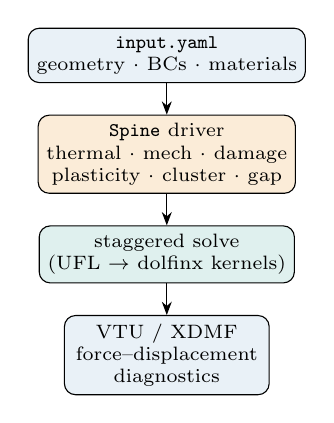
\begin{tikzpicture}[font=\scriptsize, node distance=4mm,
        box/.style={draw, rounded corners, fill=z3blue!10, minimum width=26mm, align=center, inner sep=3pt}]
        \node[box] (yaml) {\texttt{input.yaml}\\geometry $\cdot$ BCs $\cdot$ materials};
        \node[box, fill=z3amber!20, below=of yaml] (spine) {\texttt{Spine} driver\\thermal $\cdot$ mech $\cdot$ damage\\plasticity $\cdot$ cluster $\cdot$ gap};
        \node[box, fill=z3teal!15, below=of spine] (solve) {staggered solve\\(UFL $\to$ dolfinx kernels)};
        \node[box, below=of solve] (out) {VTU / XDMF\\force--displacement\\diagnostics};
        \draw[-{Stealth}] (yaml) -- (spine);
        \draw[-{Stealth}] (spine) -- (solve);
        \draw[-{Stealth}] (solve) -- (out);
      \end{tikzpicture}
    \end{column}
  \end{columns}
\end{frame}

% ---------------------------------------------------------------- 4
\begin{frame}[fragile]{The core idea: write the energy, get everything else}
  A constitutive model is a \alert{strain-energy density}; UFL's automatic
  differentiation gives the stress and the consistent tangent.
  \vspace{0.2em}
  \begin{lstlisting}
F   = ufl.variable(I + grad(u))                  # deformation gradient
psi = (mu/2)*(Ic - 3) - mu*ufl.ln(J) \
      + (lmbda/2)*ufl.ln(J)**2                    # neo-Hookean energy
P   = ufl.diff(psi, F)                            # 1st Piola-Kirchhoff = d psi / d F
R   = ufl.inner(grad(v), P) * dx                  # residual
Jac = ufl.derivative(R, u, du)                    # consistent tangent -- also AD
  \end{lstlisting}
  \begin{itemize}
    \item \texttt{P = ufl.diff(psi, F)} is the stress; \texttt{ufl.derivative} the Newton tangent -- no analytic Jacobian, ever
    \item one path for all: elasticity, hyperelasticity, J2 \alert{and crystal} plasticity, phase-field
    \item \alert{$\Rightarrow$ this is why z3st exists:} the \alert{whole coupled apparatus} is assembled once on this path and driven by YAML -- never re-derived, never re-wired
  \end{itemize}
\end{frame}

% ---------------------------------------------------------------- 5
\begin{frame}{Coupled thermo-mechanics, solved in a staggered loop}
  \small
  \begin{columns}[T]
    \begin{column}{0.56\textwidth}
      Per load step, the driver alternates until each field converges:
      \begin{enumerate}
        \item \textbf{thermal} $\;\rho c_p \dot T = \nabla\!\cdot(k(T)\nabla T) + q'''$
        \item \textbf{mechanical} $\;\nabla\!\cdot\sigma = 0$; elastic strain minus
              \alert{eigenstrains} (thermal, swelling, \alert{creep})\\
              $\varepsilon_{el} = \varepsilon(u) - \varepsilon_{th} - \varepsilon_{sw} - \varepsilon^{cr}$
        \item \textbf{damage} driven by $\psi^+(\varepsilon_{el})$, irreversible
      \end{enumerate}
      \vspace{0.5em}
      \alert{Adaptive relaxation}: per-field factors grow when the residual
      shrinks, shrink when it oscillates -- robust without a monolithic Newton.
      \vspace{0.3em}

      {\scriptsize \alert{Adaptive time-stepping} (opt-in): a stalled step rolls
      back to the last converged state and bisects $\Delta t$ -- it pushes through
      a stiff interval instead of failing.}
    \end{column}
    \begin{column}{0.44\textwidth}
      \centering
      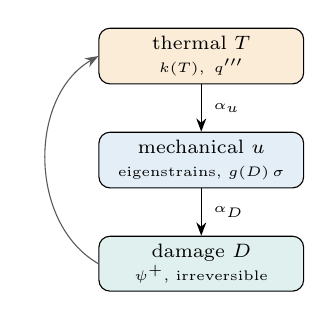
\begin{tikzpicture}[font=\scriptsize, node distance=6mm,
        s/.style={draw, rounded corners, minimum width=26mm, align=center, inner sep=3pt}]
        \node[s, fill=z3amber!20] (t) {thermal $T$\\{\tiny $k(T),\;q'''$}};
        \node[s, fill=z3blue!12, below=of t] (m) {mechanical $u$\\{\tiny eigenstrains, $g(D)\,\sigma$}};
        \node[s, fill=z3teal!15, below=of m] (d) {damage $D$\\{\tiny $\psi^+$, irreversible}};
        \draw[-{Stealth}] (t) -- node[right=1pt]{\tiny $\alpha_u$} (m);
        \draw[-{Stealth}] (m) -- node[right=1pt]{\tiny $\alpha_D$} (d);
        \draw[-{Stealth}, z3grey] (d.west) to[bend left=60] (t.west);
      \end{tikzpicture}\\[3pt]
      {\tiny staggered loop -- under-relax each field, repeat until all converge}
      \vspace{0.6em}

      {\scriptsize Damage degrades the stress -- thermal-stress included --
      via a consistent $g(D)$; essential for tractable thermal-shock fracture.}
    \end{column}
  \end{columns}
\end{frame}

% ---------------------------------------------------------------- 6
\begin{frame}{Coupled multi-physics -- and across separate bodies}
  \begin{columns}[T]
    \begin{column}{0.5\textwidth}
      \textbf{Coupled physics in one solve}
      \begin{itemize}
        \item thermal $+$ mechanical $+$ damage / phase-field, two-way coupled
        \item temperature drives thermal strain and stress
        \item damage degrades the stress, thermal-stress \alert{included}
        \item phase-field: AT1 / AT2, Miehe / Amor, hybrid
      \end{itemize}
    \end{column}
    \begin{column}{0.5\textwidth}
      \textbf{Heat across bodies: gap conductance}
      \begin{itemize}
        \item heat crosses a gap between \alert{separate bodies / regions}
        \item $h_{gap}(T_{gap})$ as a thermal interface condition
        \item e.g. fuel pellet $\to$ cladding -- essential for fuel-performance modelling
      \end{itemize}
    \end{column}
  \end{columns}
  \vspace{0.7em}
  \begin{block}{}
    \footnotesize
    \alert{New / exploratory:} cluster dynamics -- defect-population evolution in
    cluster-size space ($\partial_t c = -v\,\partial_n c + D\,\partial_{nn} c$).
    Implemented, not yet investigated; a path towards a genuine micro-to-continuum link.
  \end{block}
\end{frame}

% ---------------------------------------------------------------- 6b (PCMI -- fuel rod)
\begin{frame}{Pellet--cladding interaction (PCMI) over a full irradiation}
  \centering
  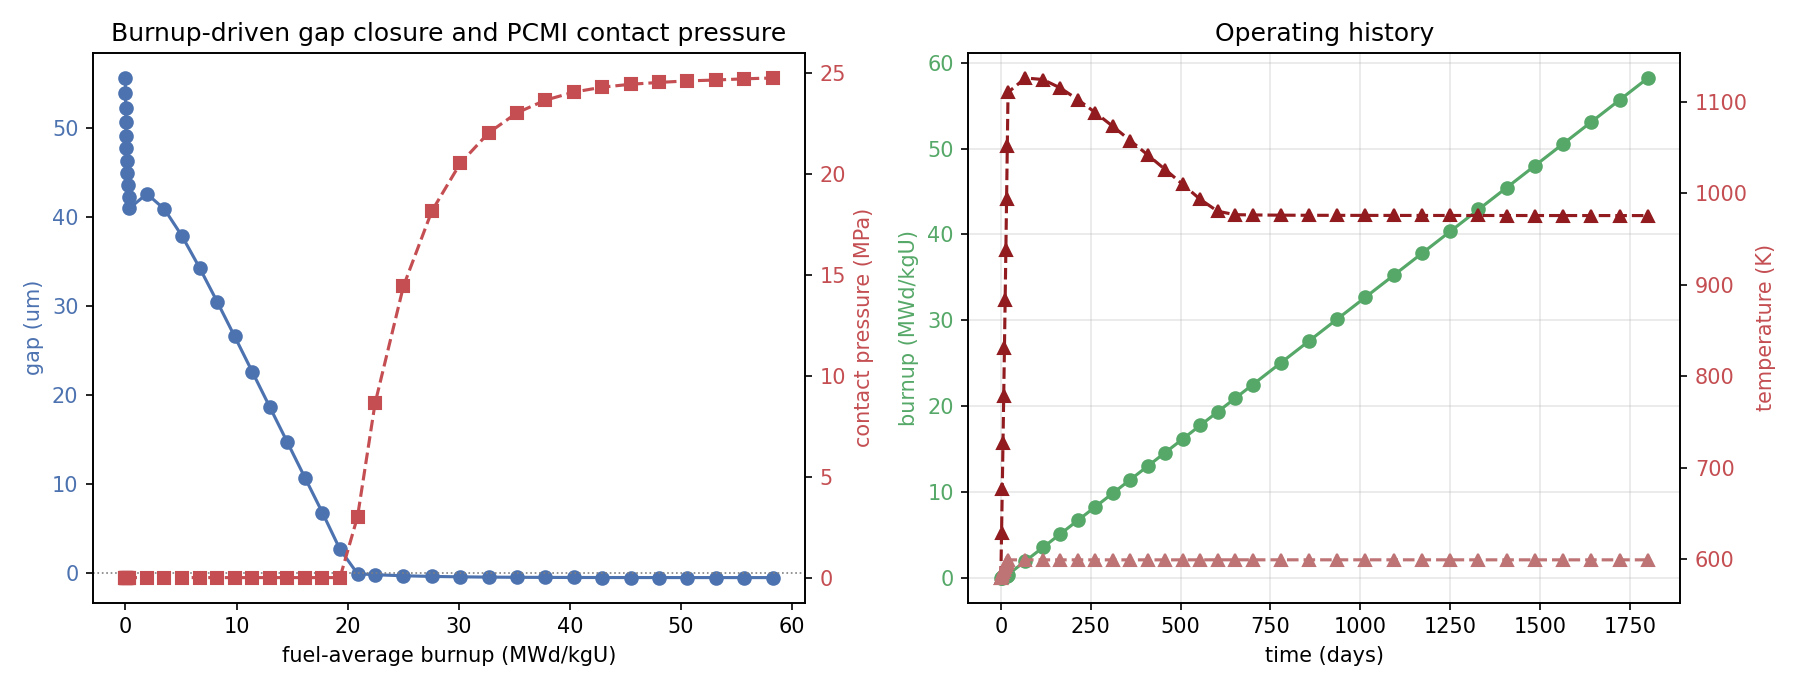
\includegraphics[width=0.86\textwidth]{figures/pcmi_burnup_curves.png}\\[3pt]
  \footnotesize
  \begin{columns}[T]
    \begin{column}{0.5\textwidth}
      \begin{itemize}
        \item fuel swells with burnup and \alert{closes the gap} ($\sim$21\,MWd/kgU)
        \item contact pressure \alert{emerges} (explicit penalty) and
              \alert{creep-saturates} near 25\,MPa
      \end{itemize}
    \end{column}
    \begin{column}{0.5\textwidth}
      \begin{itemize}
        \item contact raises gap conductance -- peak fuel $T$ \alert{drops}
              1126 $\to$ 976\,K (two-way feedback)
        \item one \texttt{input.yaml}: $k(T)$, swelling, creep, gap, contact;
              verified vs Lam\'e (backup)
      \end{itemize}
    \end{column}
  \end{columns}
\end{frame}

% ---------------------------------------------------------------- 7
\begin{frame}{Verified, reproducible, and easy to drive}
  \small
  \begin{columns}[T]
    \begin{column}{0.5\textwidth}
      \textbf{Verified -- every solver, every physics}
      \begin{itemize}
        \item $\sim$45 cases, each checked numerically against an \alert{analytical} solution
        \item thermal, mechanical, plasticity, fracture -- all covered
        \item fast subset in \alert{CI on every push}; full suite run locally
      \end{itemize}
      \vspace{0.4em}
      \textbf{Teaching cases}
      \begin{itemize}
        \item 1D bar and the same bar in full 3D
        \item identical $u(L)=PL/E$ -- pick a regime, don't rewrite the model
      \end{itemize}
    \end{column}
    \begin{column}{0.5\textwidth}
      \textbf{Made for experiments}
      \begin{itemize}
        \item \alert{hot reload}: edit tolerances / relaxation mid-run
        \item per-step force--displacement streaming
        \item matrix diagnostics, structured logs
      \end{itemize}
      \vspace{0.2em}
      \centering
      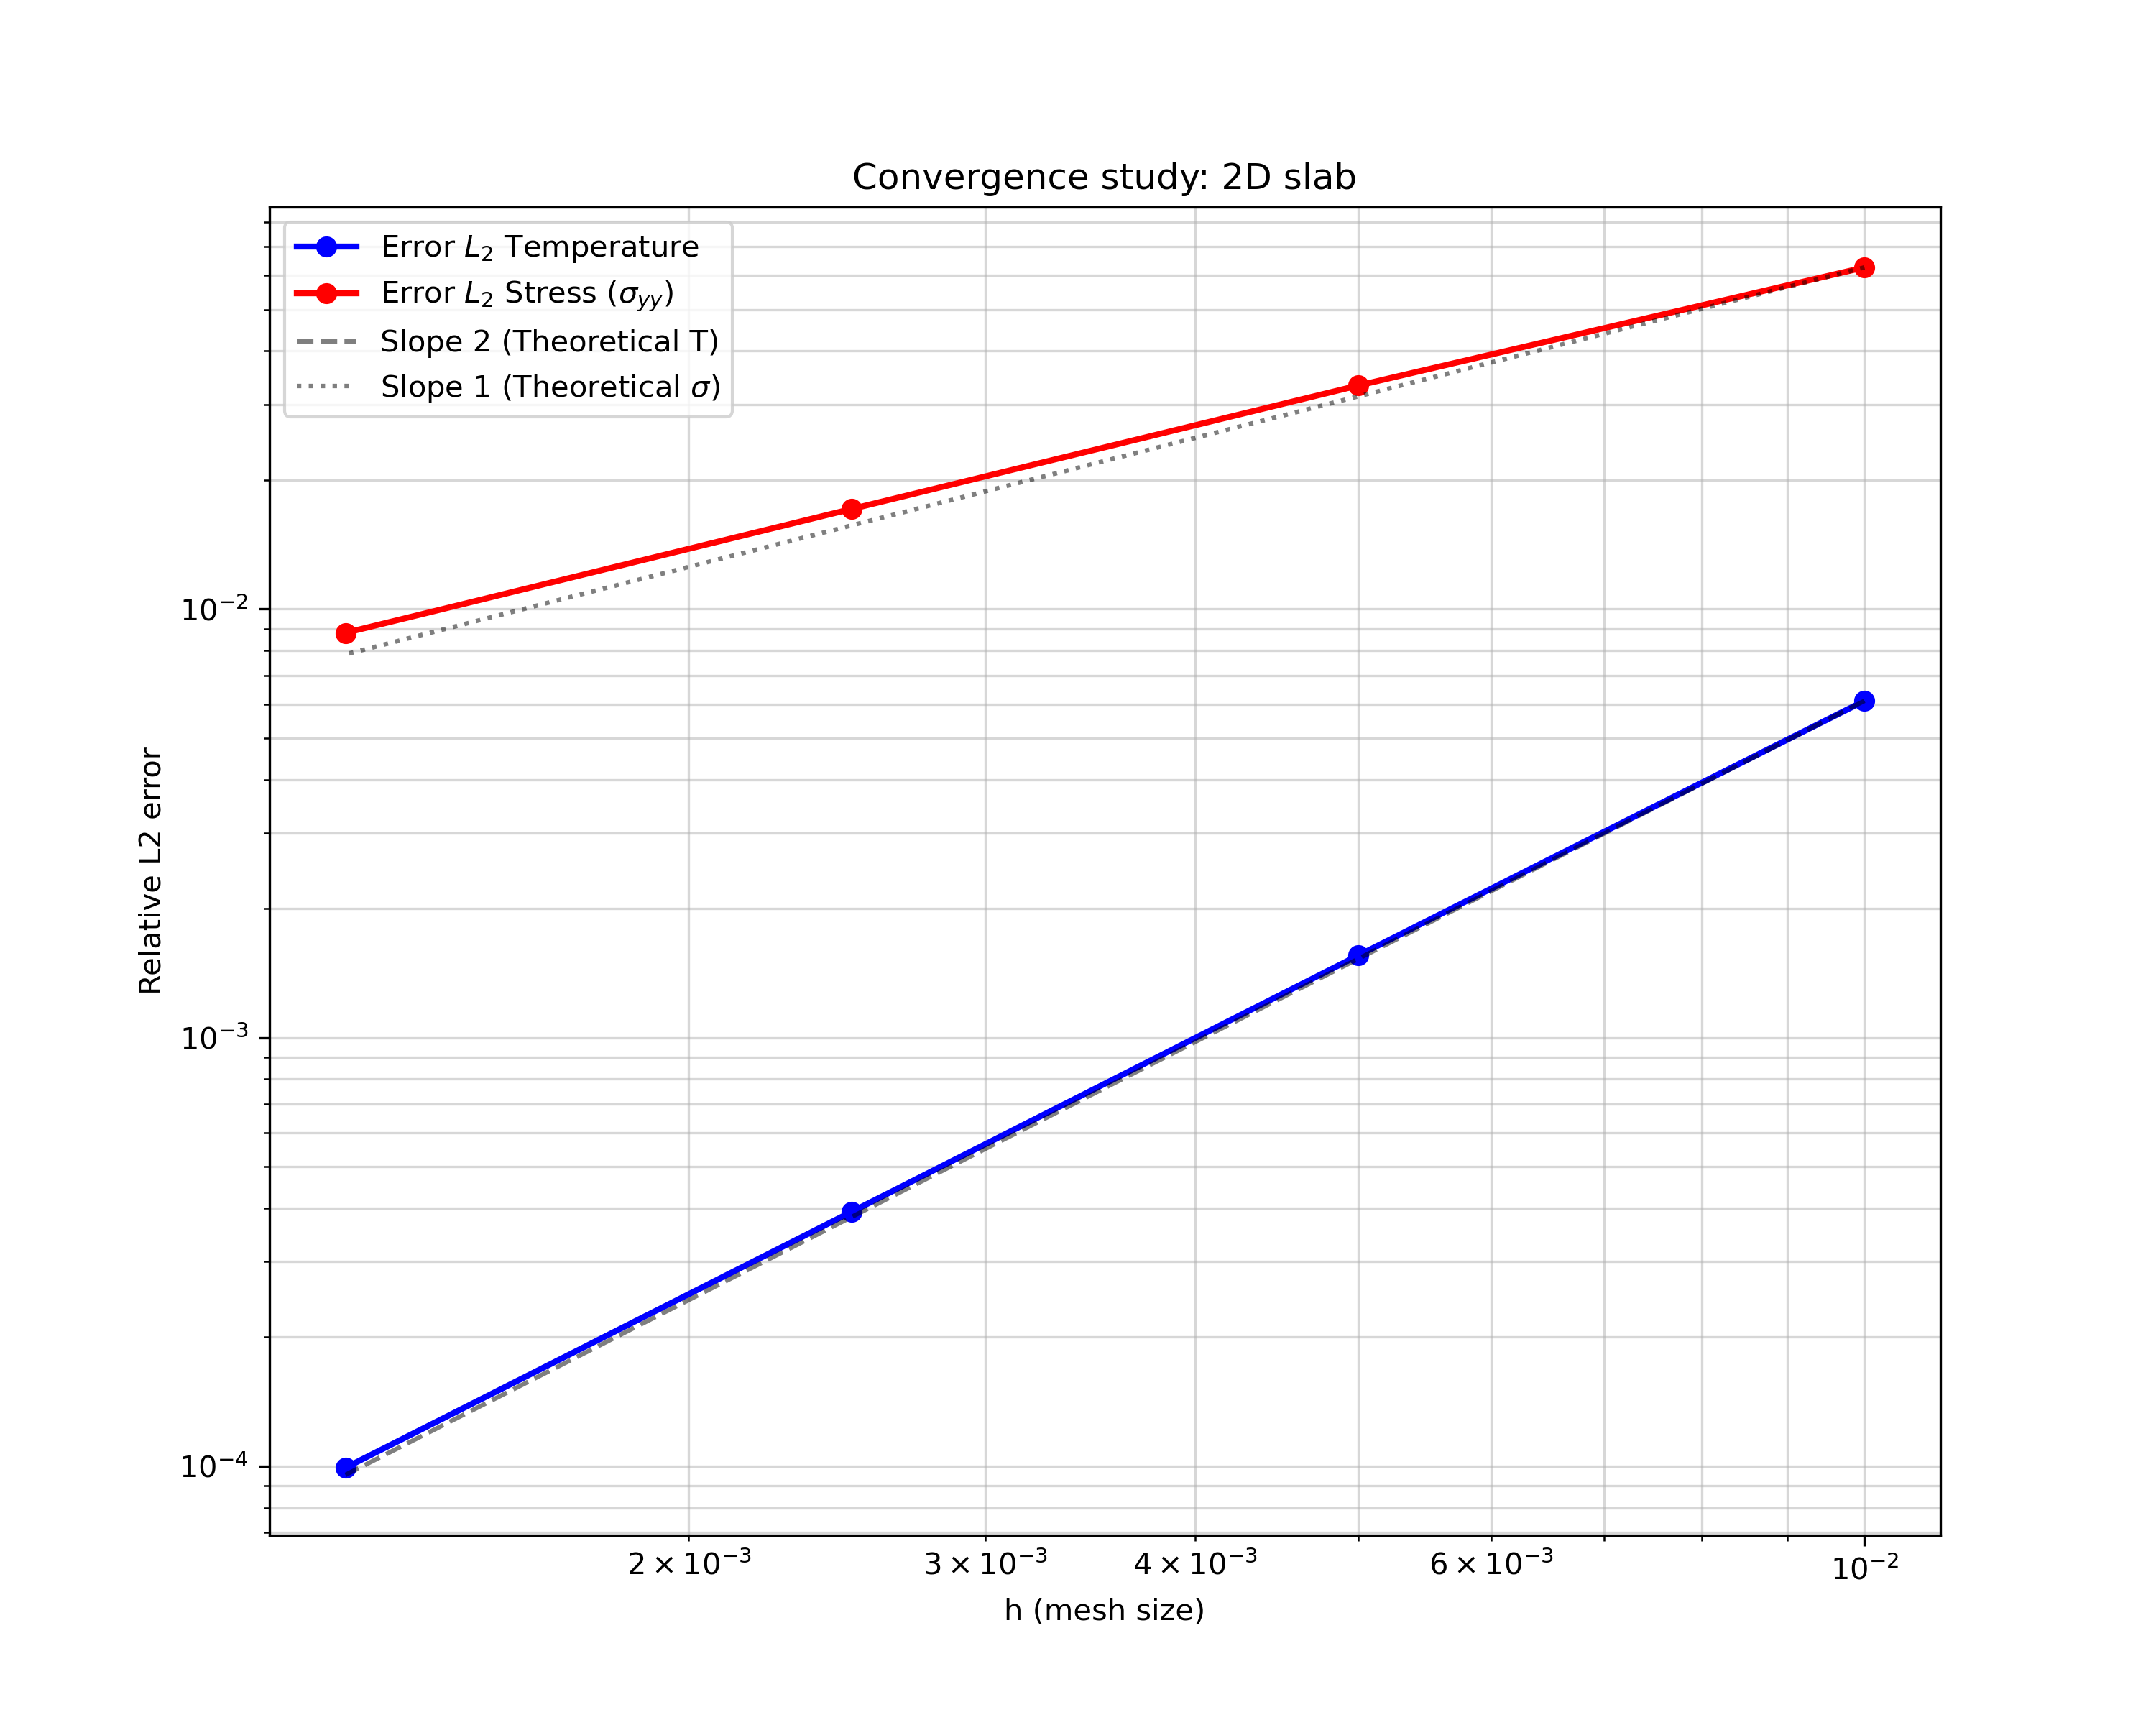
\includegraphics[width=0.58\textwidth]{figures/convergence_study.png}\\
      {\scriptsize $L_2$ error at the theoretical rates ($T$: 2, $\sigma$: 1)}
    \end{column}
  \end{columns}
\end{frame}

% ---------------------------------------------------------------- 8
\begin{frame}{Hero case: thermal-shock cracking of a UO\textsubscript{2} pellet}
  \begin{columns}[T]
    \begin{column}{0.34\textwidth}
      A cold-contact wedge cools the rim of a hot disc; the tensile hoop-stress
      ring it sets up drives \alert{discrete radial cracks} -- as observed in a
      real UO\textsubscript{2} pellet.
      \vspace{0.4em}
      \begin{itemize}\small
        \item 2D plane-strain half-disc, mirror symmetry
        \item AT1 $+$ Amor $+$ hybrid
        \item fully coupled $T \to \varepsilon_{el} \to D$
      \end{itemize}
      \vspace{0.3em}
      {\scriptsize One \texttt{input.yaml}; every ingredient on the previous slides
      meets here.}
    \end{column}
    \begin{column}{0.66\textwidth}
      \centering
      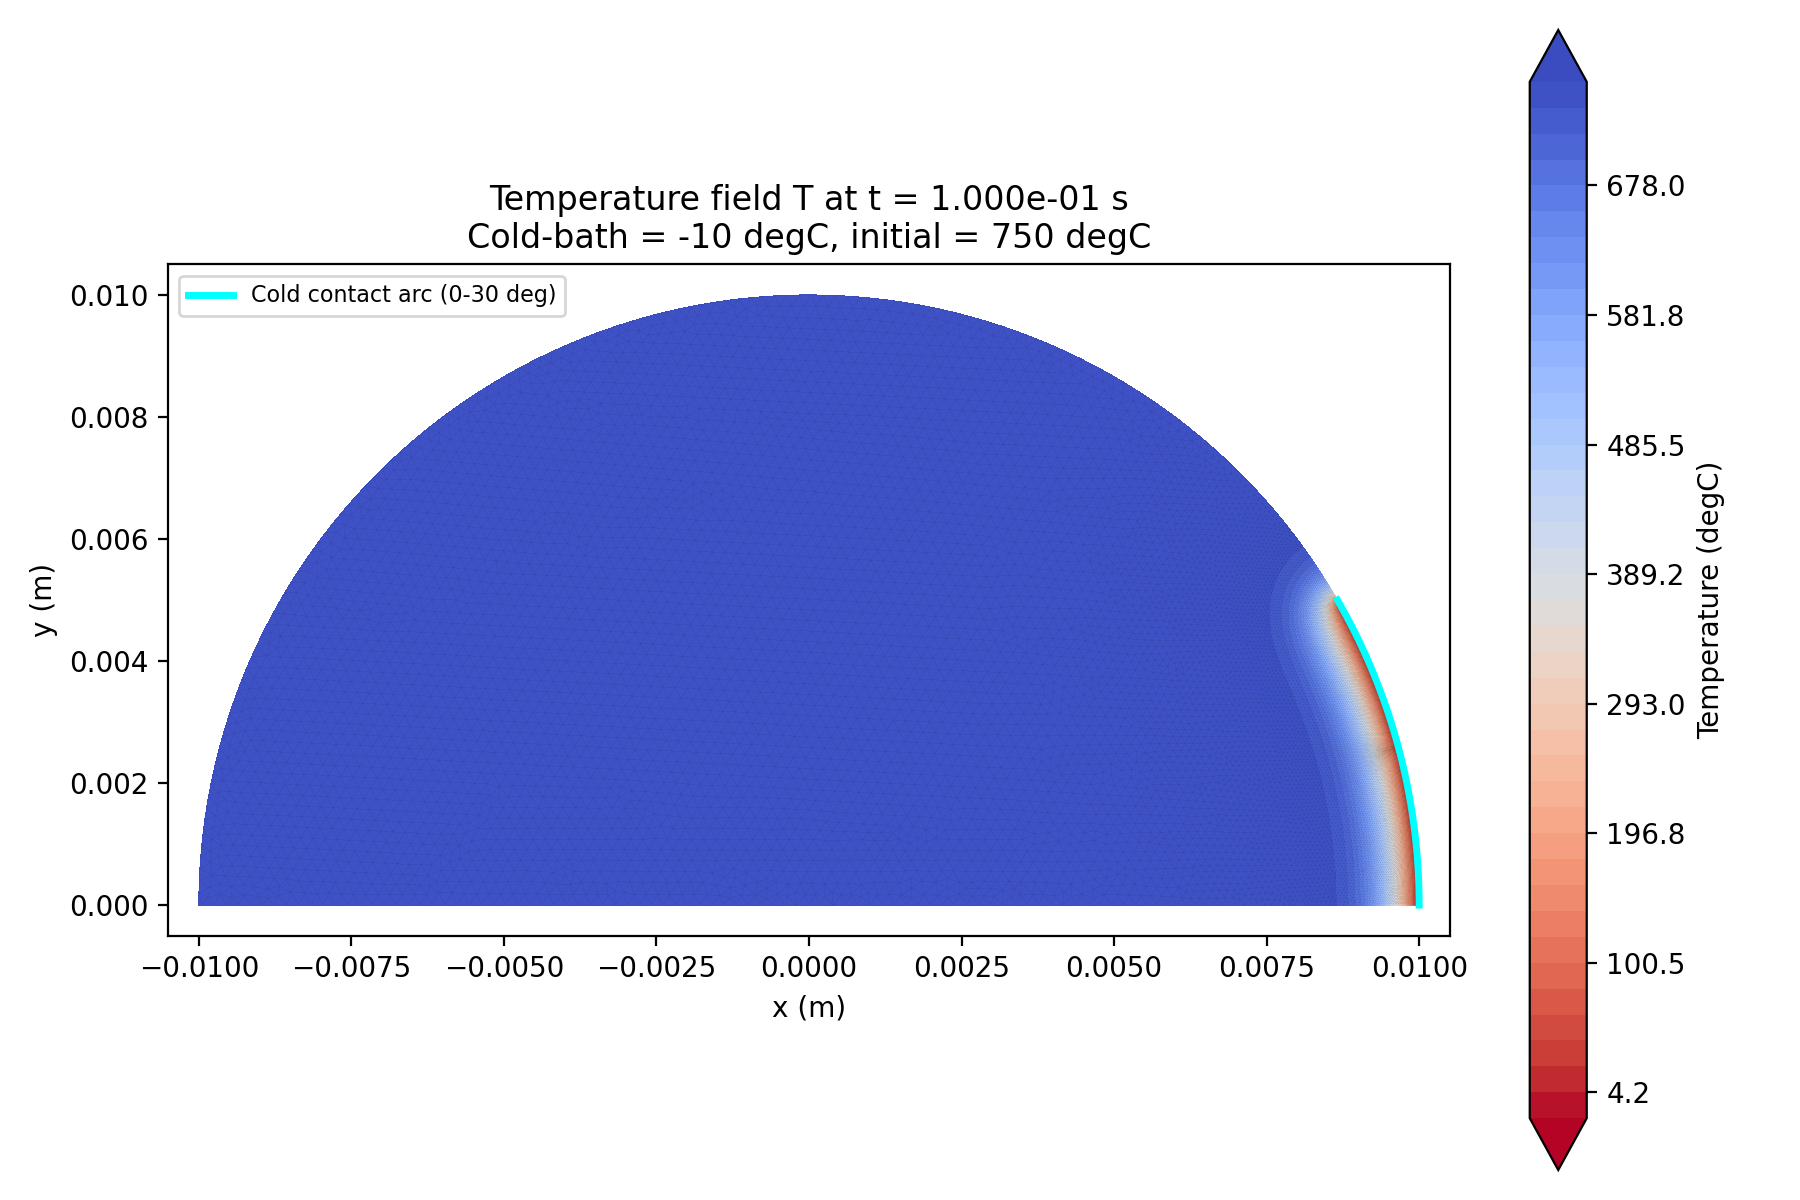
\includegraphics[width=0.47\textwidth]{figures/case14_temperature.png}\hfill
      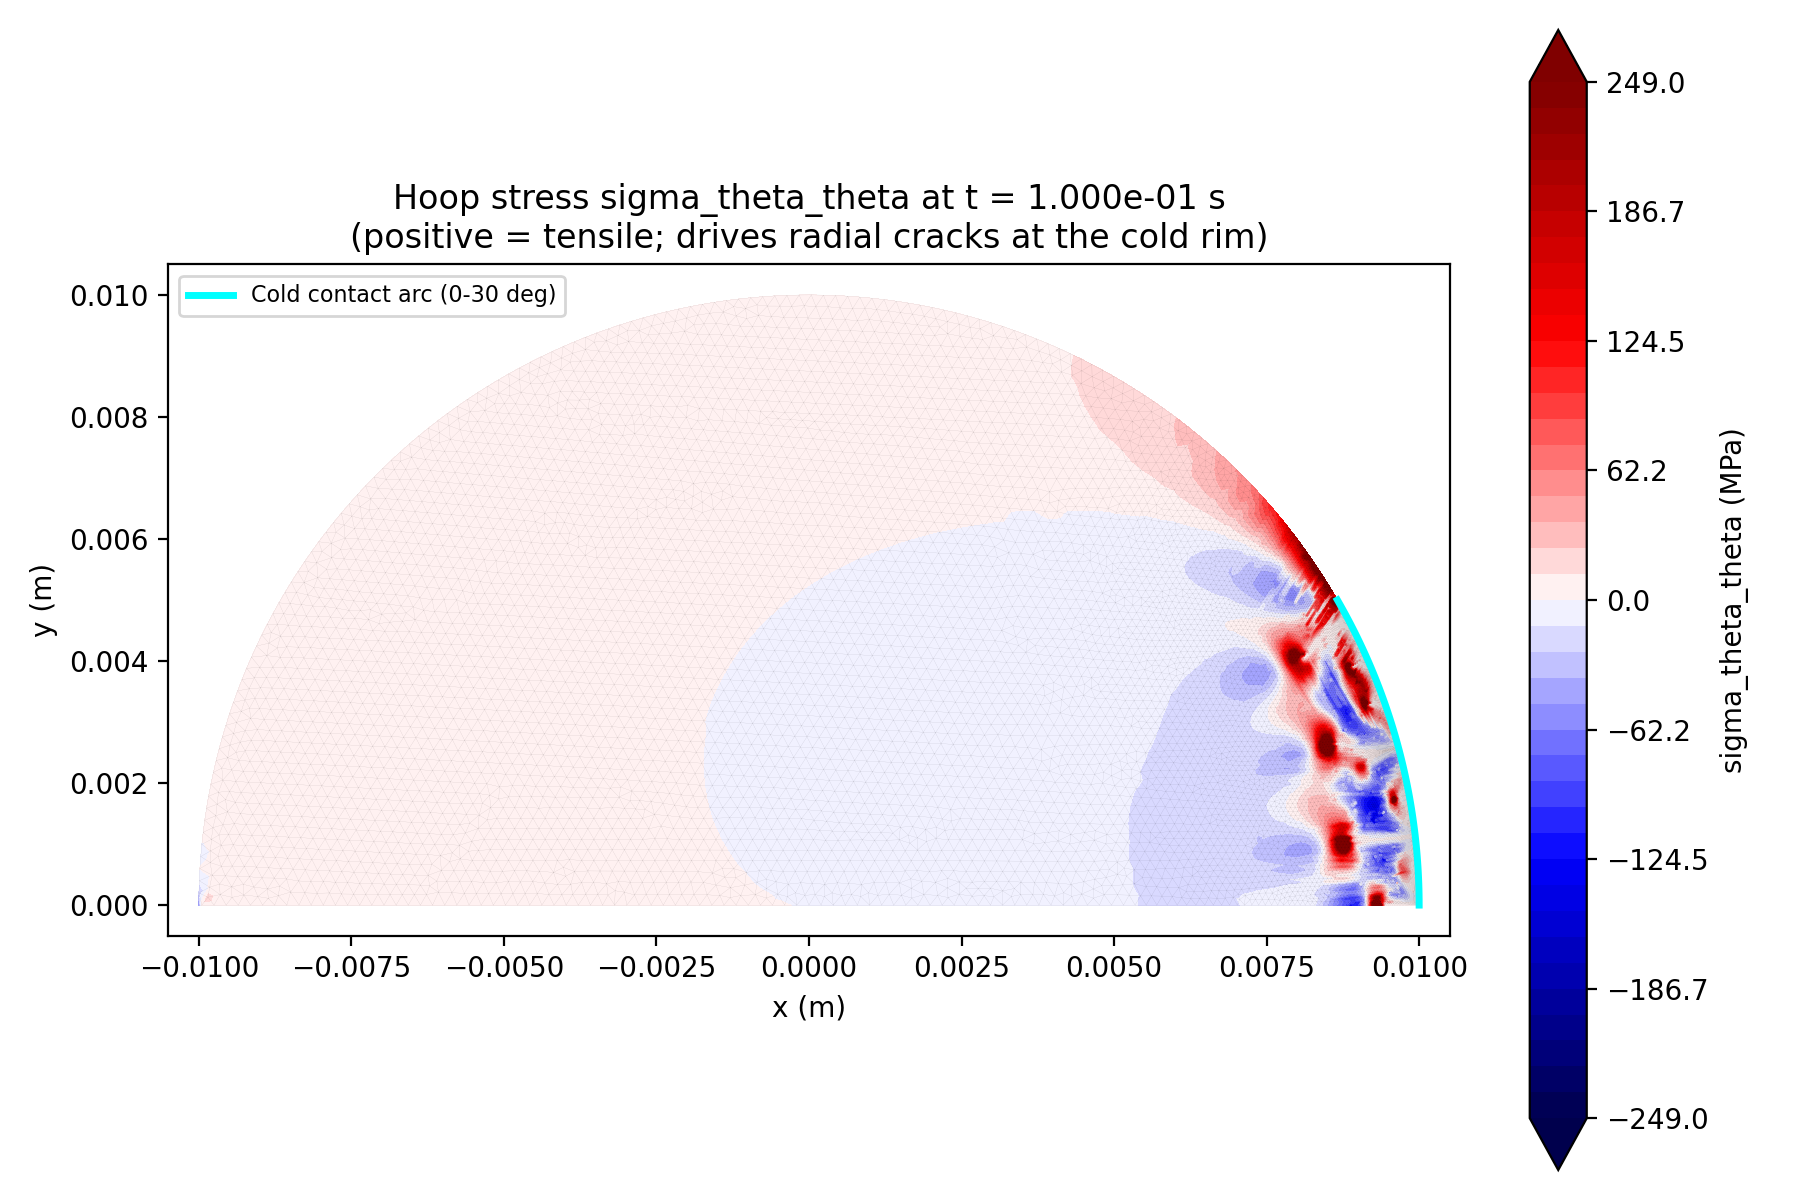
\includegraphics[width=0.47\textwidth]{figures/case14_hoop.png}\\[2pt]
      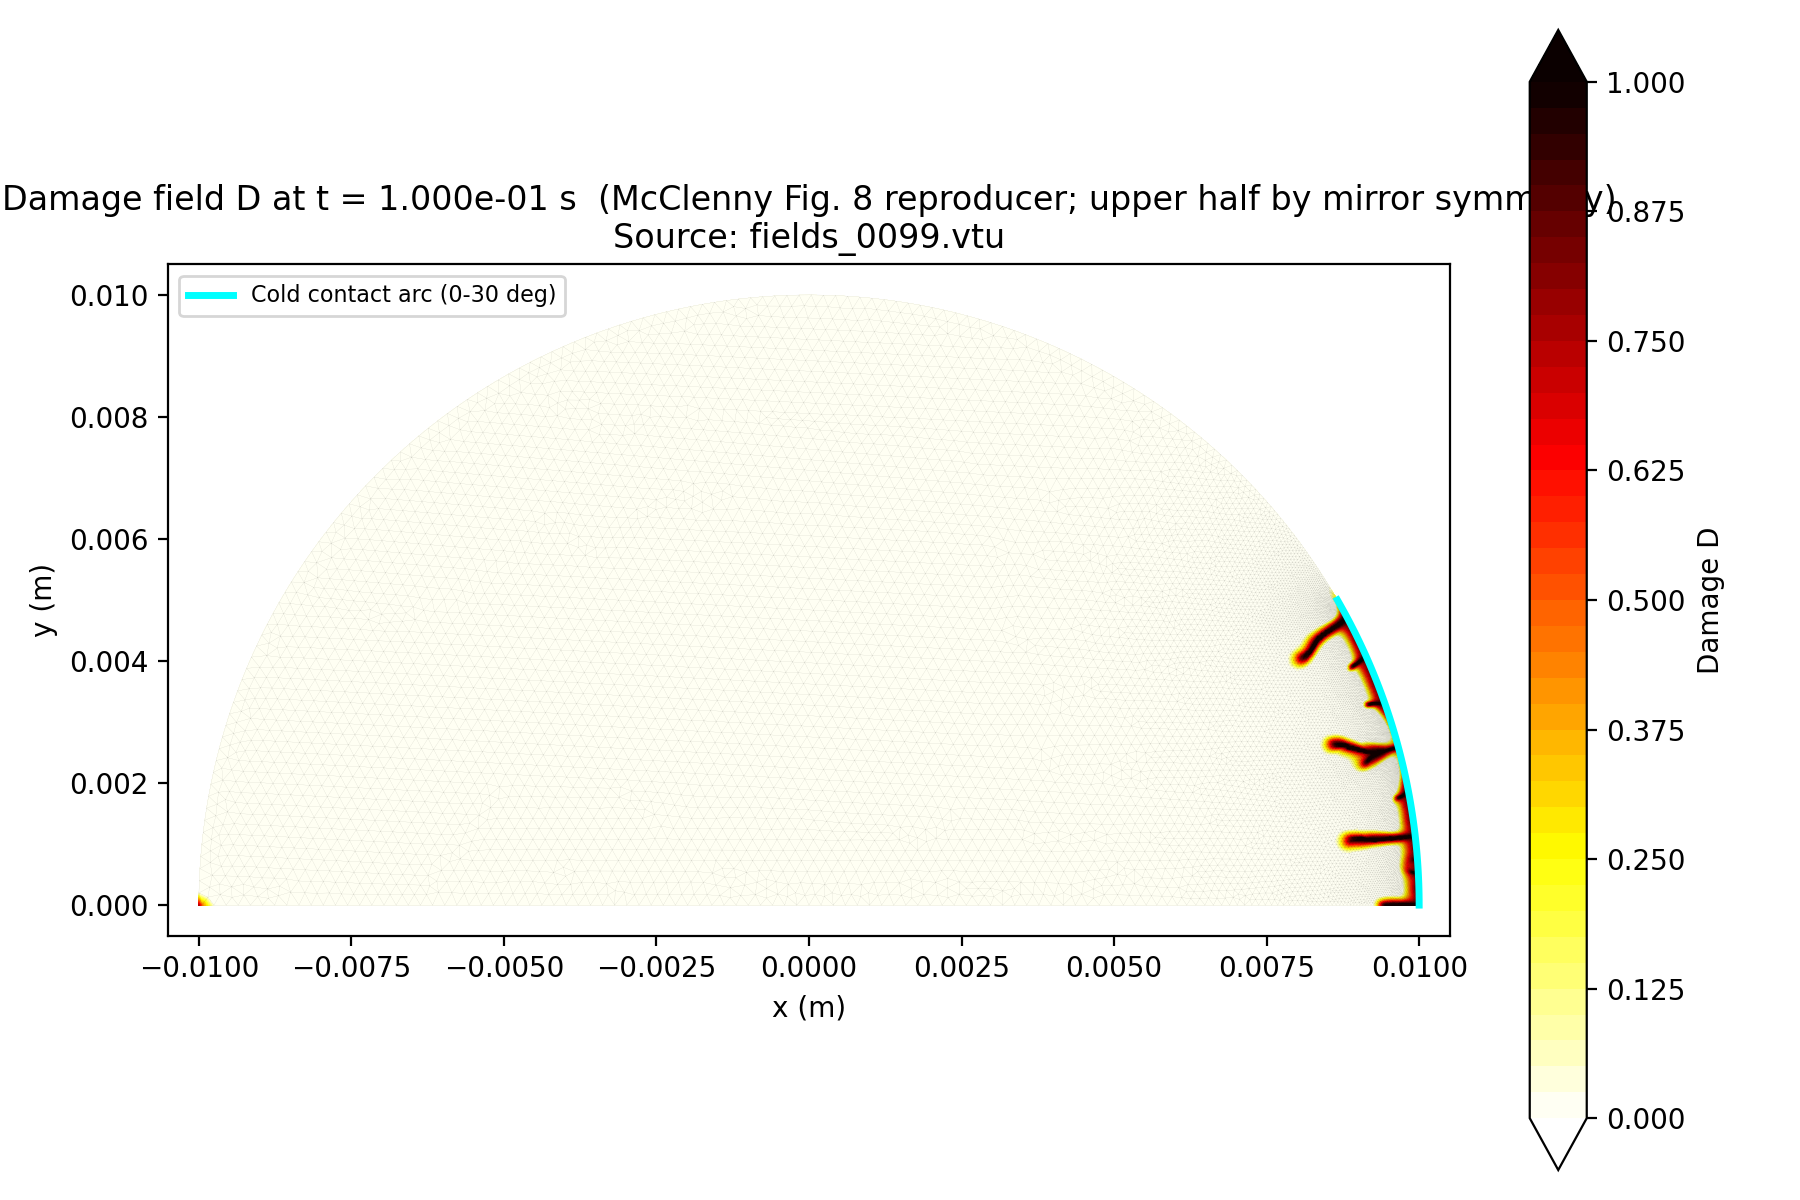
\includegraphics[width=0.47\textwidth]{figures/case14_damage.png}\hfill
      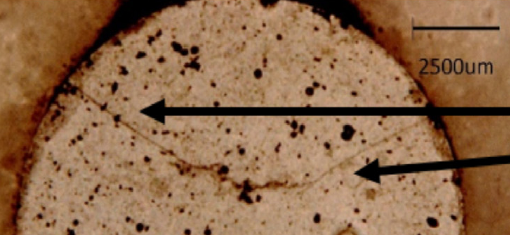
\includegraphics[width=0.47\textwidth]{figures/case14_experiment.png}\\[1pt]
      {\scriptsize top: cold wedge $\to$ tensile hoop-stress ring \quad\textbar\quad
       bottom: \alert{simulated} cracks vs a \alert{real} UO\textsubscript{2} cross-section}
    \end{column}
  \end{columns}
\end{frame}

% ---------------------------------------------------------------- 9
\begin{frame}{Open, and runnable on your laptop}
  \footnotesize
  \begin{columns}[T]
    \begin{column}{0.58\textwidth}
      \textbf{Z3ST is}
      \begin{itemize}
        \item \alert{open + FEniCSx-native} -- the whole coupled apparatus, assembled for you
        \item thermo-mech-fracture across bodies; J2 + crystal plasticity; energy-first via AD
        \item YAML-driven, material-agnostic, \alert{verified} ($\sim$45 analytic cases; subset in CI)
      \end{itemize}
      \vspace{0.2em}
      \textbf{Get it / See it live}
      \begin{itemize}
        \item \texttt{github.com/giozu/z3st} \quad(Apache-2.0)
        \item docs: \texttt{giozu.github.io/z3st} \quad DOI: \texttt{10.5281/zenodo.17748028}
        \item \alert{live demo} at the poster session -- a coupled case end to end
      \end{itemize}
    \end{column}
    \begin{column}{0.42\textwidth}
      \textbf{Future developments}
      \begin{itemize}
        \item \texttt{dolfinx\_mpc} contact: per-facet pressure (axial ridging),
              periodic BCs
        \item coupling to \alert{SCIANTIX} (fission gas) and \alert{M\'erope}
              (microstructure)
        \item monolithic phase-field Newton for spontaneous nucleation
        \item full constitutive-law \alert{discovery} through the coupled adjoint
      \end{itemize}
    \end{column}
  \end{columns}
  \vspace{0.1em}
  \centering
  {\scriptsize Already in use at PoliMi: grant proposals (irradiated materials, coated
  claddings, advanced fuels; Euratom calls), three student projects, didactic support.}\\[2pt]
  \alert{\large Thank you -- questions welcome.}\\[2pt]
  {\scriptsize \texttt{giovanni.zullo@polimi.it}}
\end{frame}

% ---------------------------------------------------------------- backup
\appendix
\begin{frame}[fragile]{Backup: the staggered solver, in one screen}
\begin{lstlisting}
for iteration in range(max_iter):
    conv_th,   _ = self._thermal_step(...)       # k(T), q''' , transient
    conv_mech, _ = self._mechanical_step(...)    # eigenstrain, g(D)*sigma
    self.update_history(u_new, T=T_new)          # phase-field driver psi+
    conv_dmg,  _ = self._damage_step(...)        # irreversible D
    if conv_th and conv_mech and conv_dmg:
        return True                              # step converged
\end{lstlisting}
\vspace{0.3em}
{\scriptsize Adaptive per-field relaxation (grow / shrink on residual trend) keeps the
fixed-point iteration stable across linear elasticity through thermal-shock fracture.}
\end{frame}

\begin{frame}{Backup: constitutive models available}
  \centering
  \begin{tabular}{@{}ll@{}}
    \toprule
    Model & Path \\
    \midrule
    Isotropic elasticity (Lam\'e) & $\sigma = \lambda\,\mathrm{tr}(\varepsilon)I + 2G\varepsilon$ \\
    Anisotropic (Voigt) & $\sigma = C:\varepsilon$, optional 6$\times$6 $C$ \\
    Hyperelasticity (neo-Hookean) & $P = \partial_F \psi$ (AD) \\
    J2 plasticity (macroscopic) & return mapping, linear hardening \\
    Crystal plasticity (single grain) & slip-system viscoplasticity, AD Jacobian \\
    Creep (Norton $+$ irradiation) & implicit backward-Euler return, AD tangent \\
    Eigenstrains & thermal, swelling, densification (callables) \\
    Phase-field damage & AT1 / AT2, Miehe / Amor, hybrid \\
    Custom & user Python stress callable (e.g. the CP law) \\
    \bottomrule
  \end{tabular}
\end{frame}

\begin{frame}{Backup: plasticity, verified against theory}
  \begin{columns}[T]
    \begin{column}{0.5\textwidth}
      \centering
      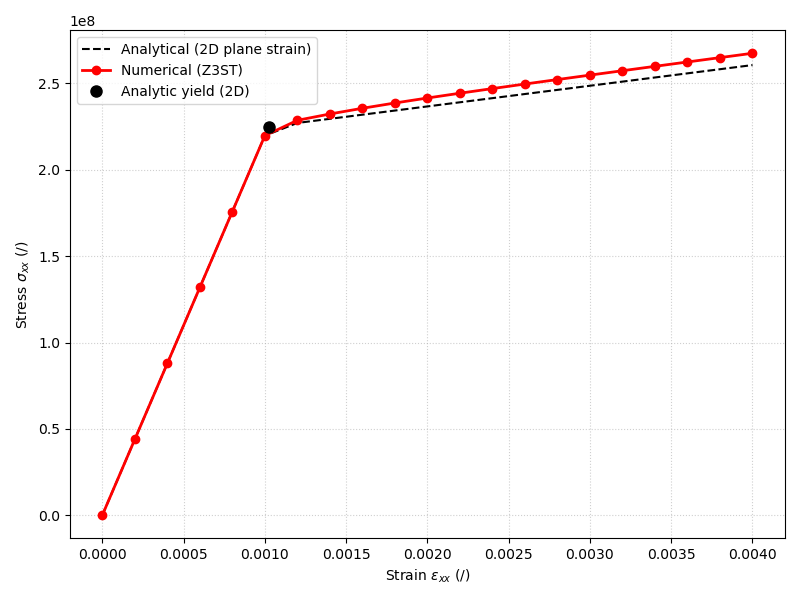
\includegraphics[width=\textwidth]{figures/j2_stress_strain.png}\\
      {\scriptsize J2 (macroscopic): numerical vs analytical 2D plane strain}
    \end{column}
    \begin{column}{0.5\textwidth}
      \centering
      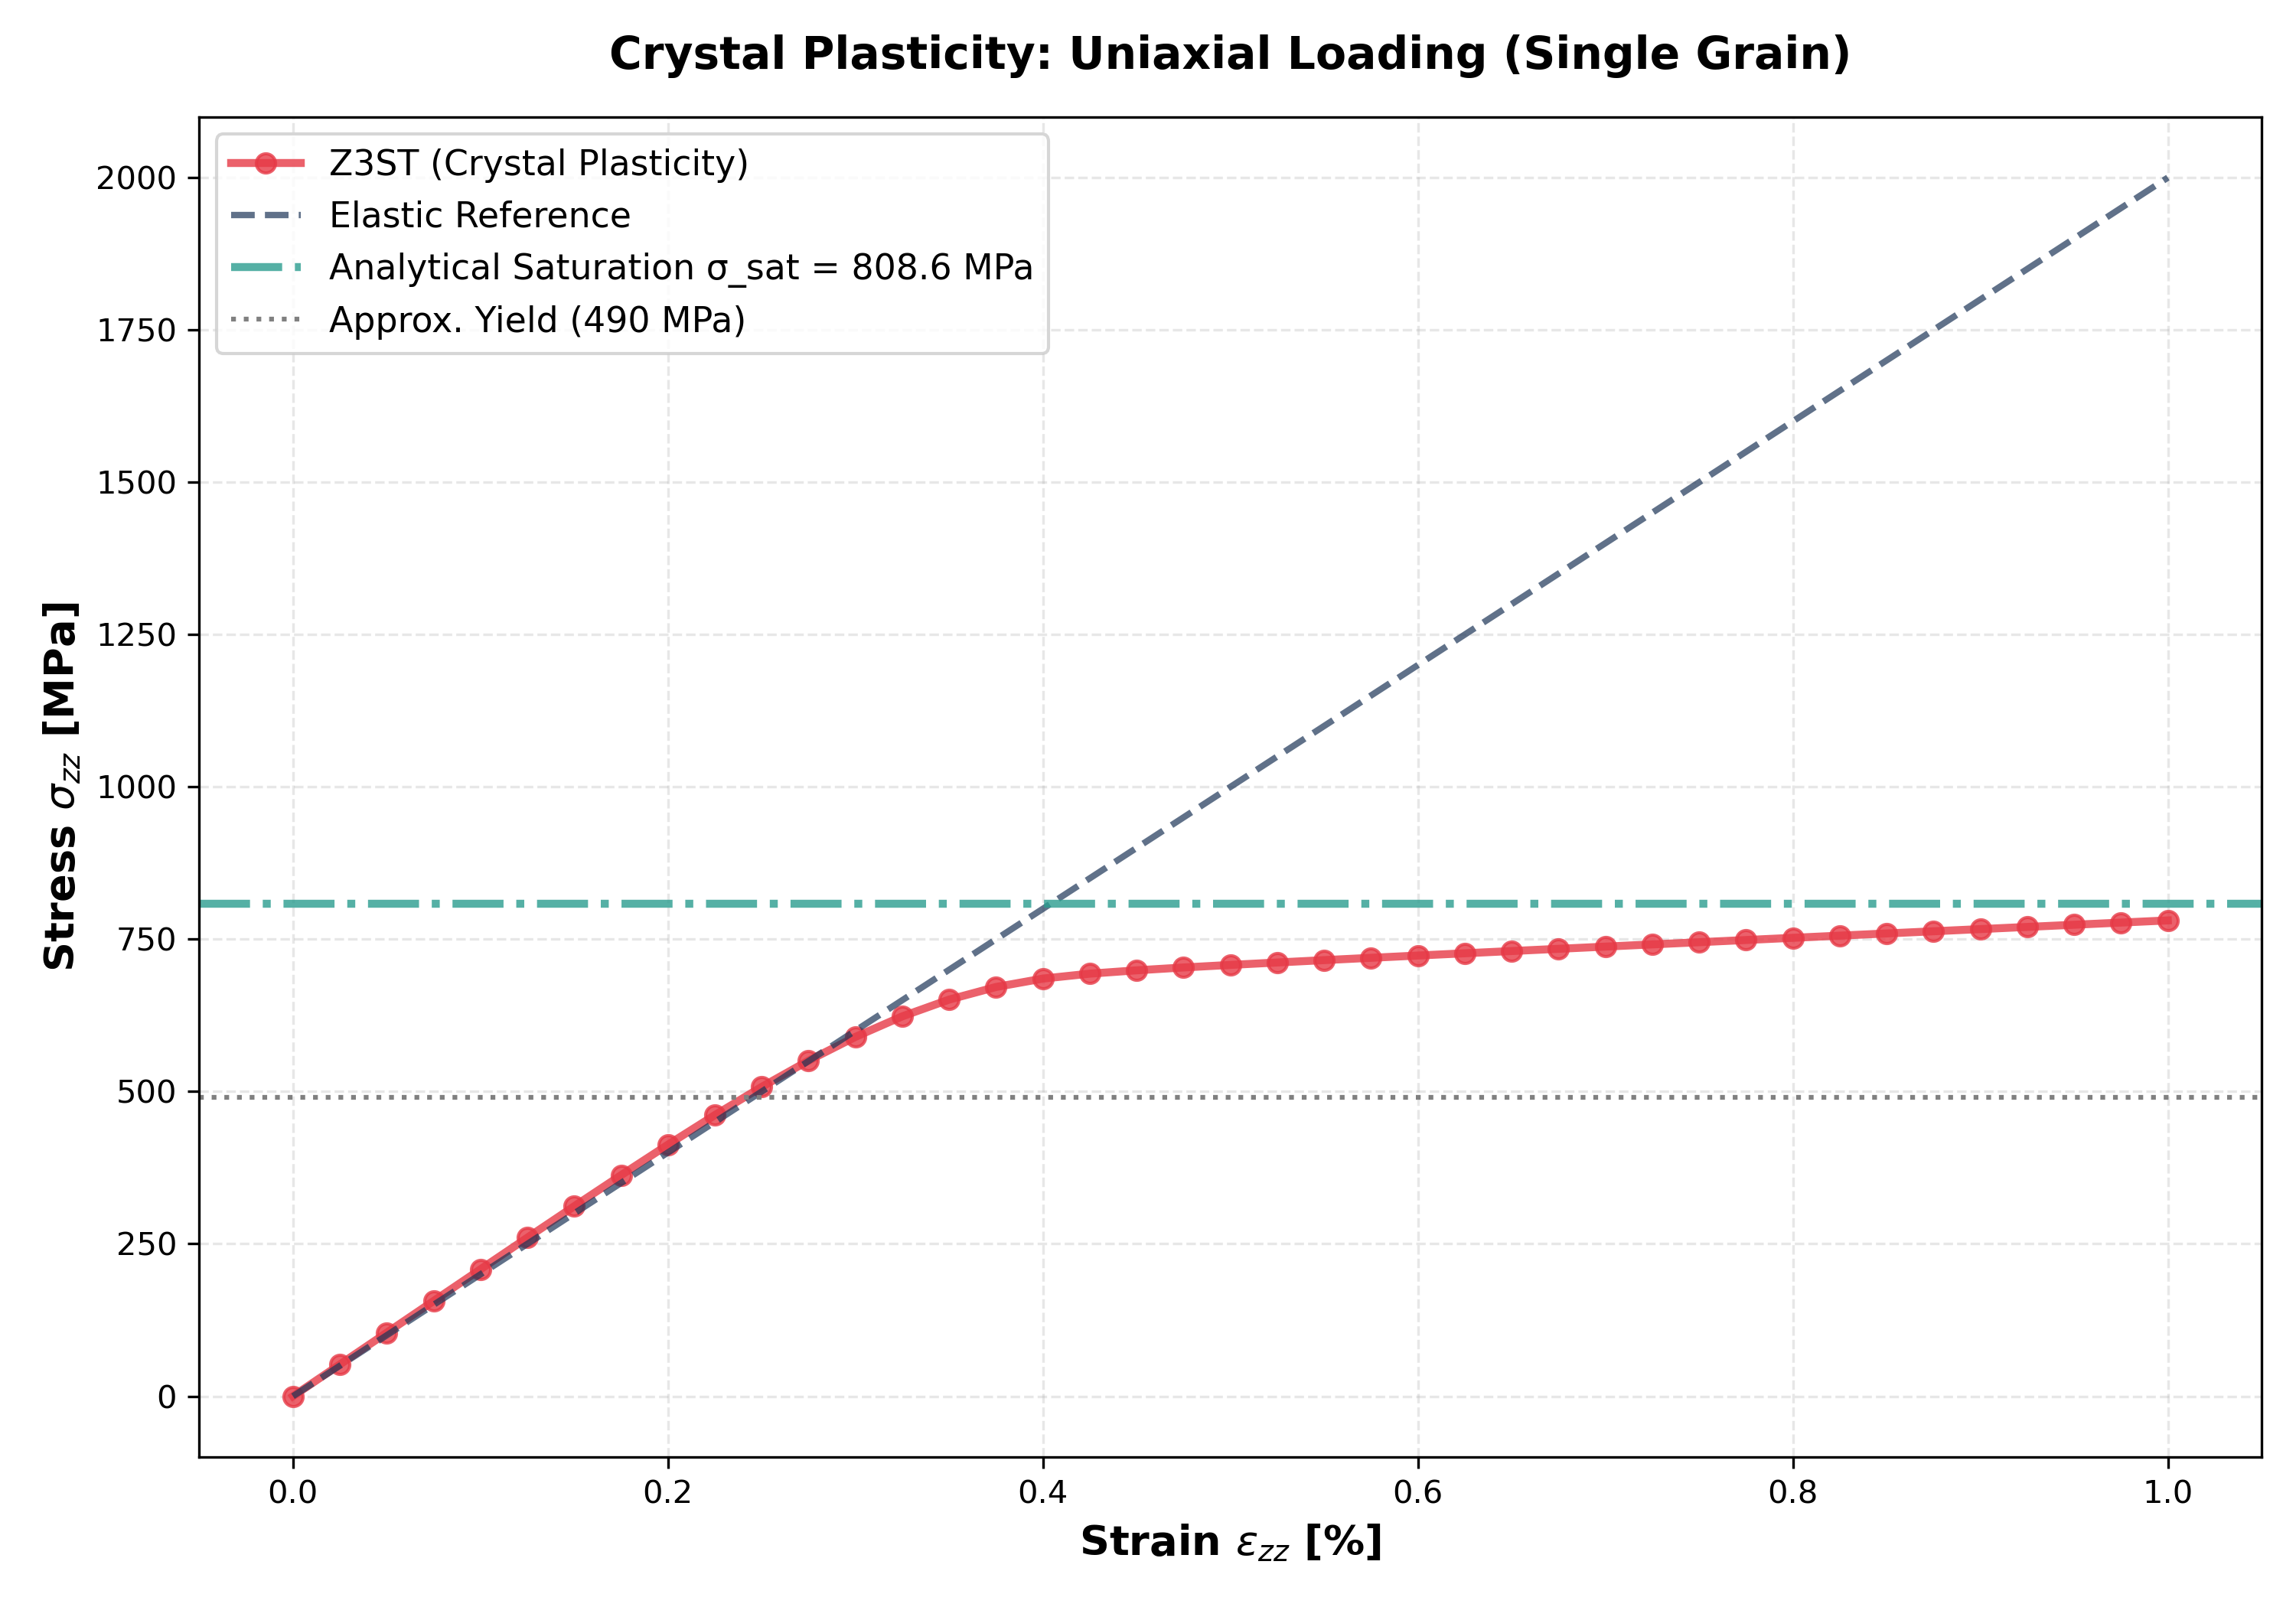
\includegraphics[width=\textwidth]{figures/cp_stress_strain.png}\\
      {\scriptsize crystal plasticity (single grain): saturates to the analytical $\sigma_{sat}$}
    \end{column}
  \end{columns}
  \vspace{0.3em}
  \centering
  {\scriptsize same AD path, two scales -- the slip-system Jacobian is differentiated automatically}
\end{frame}

\begin{frame}{Backup: coupled thermo-mechanics, verified}
  \centering
  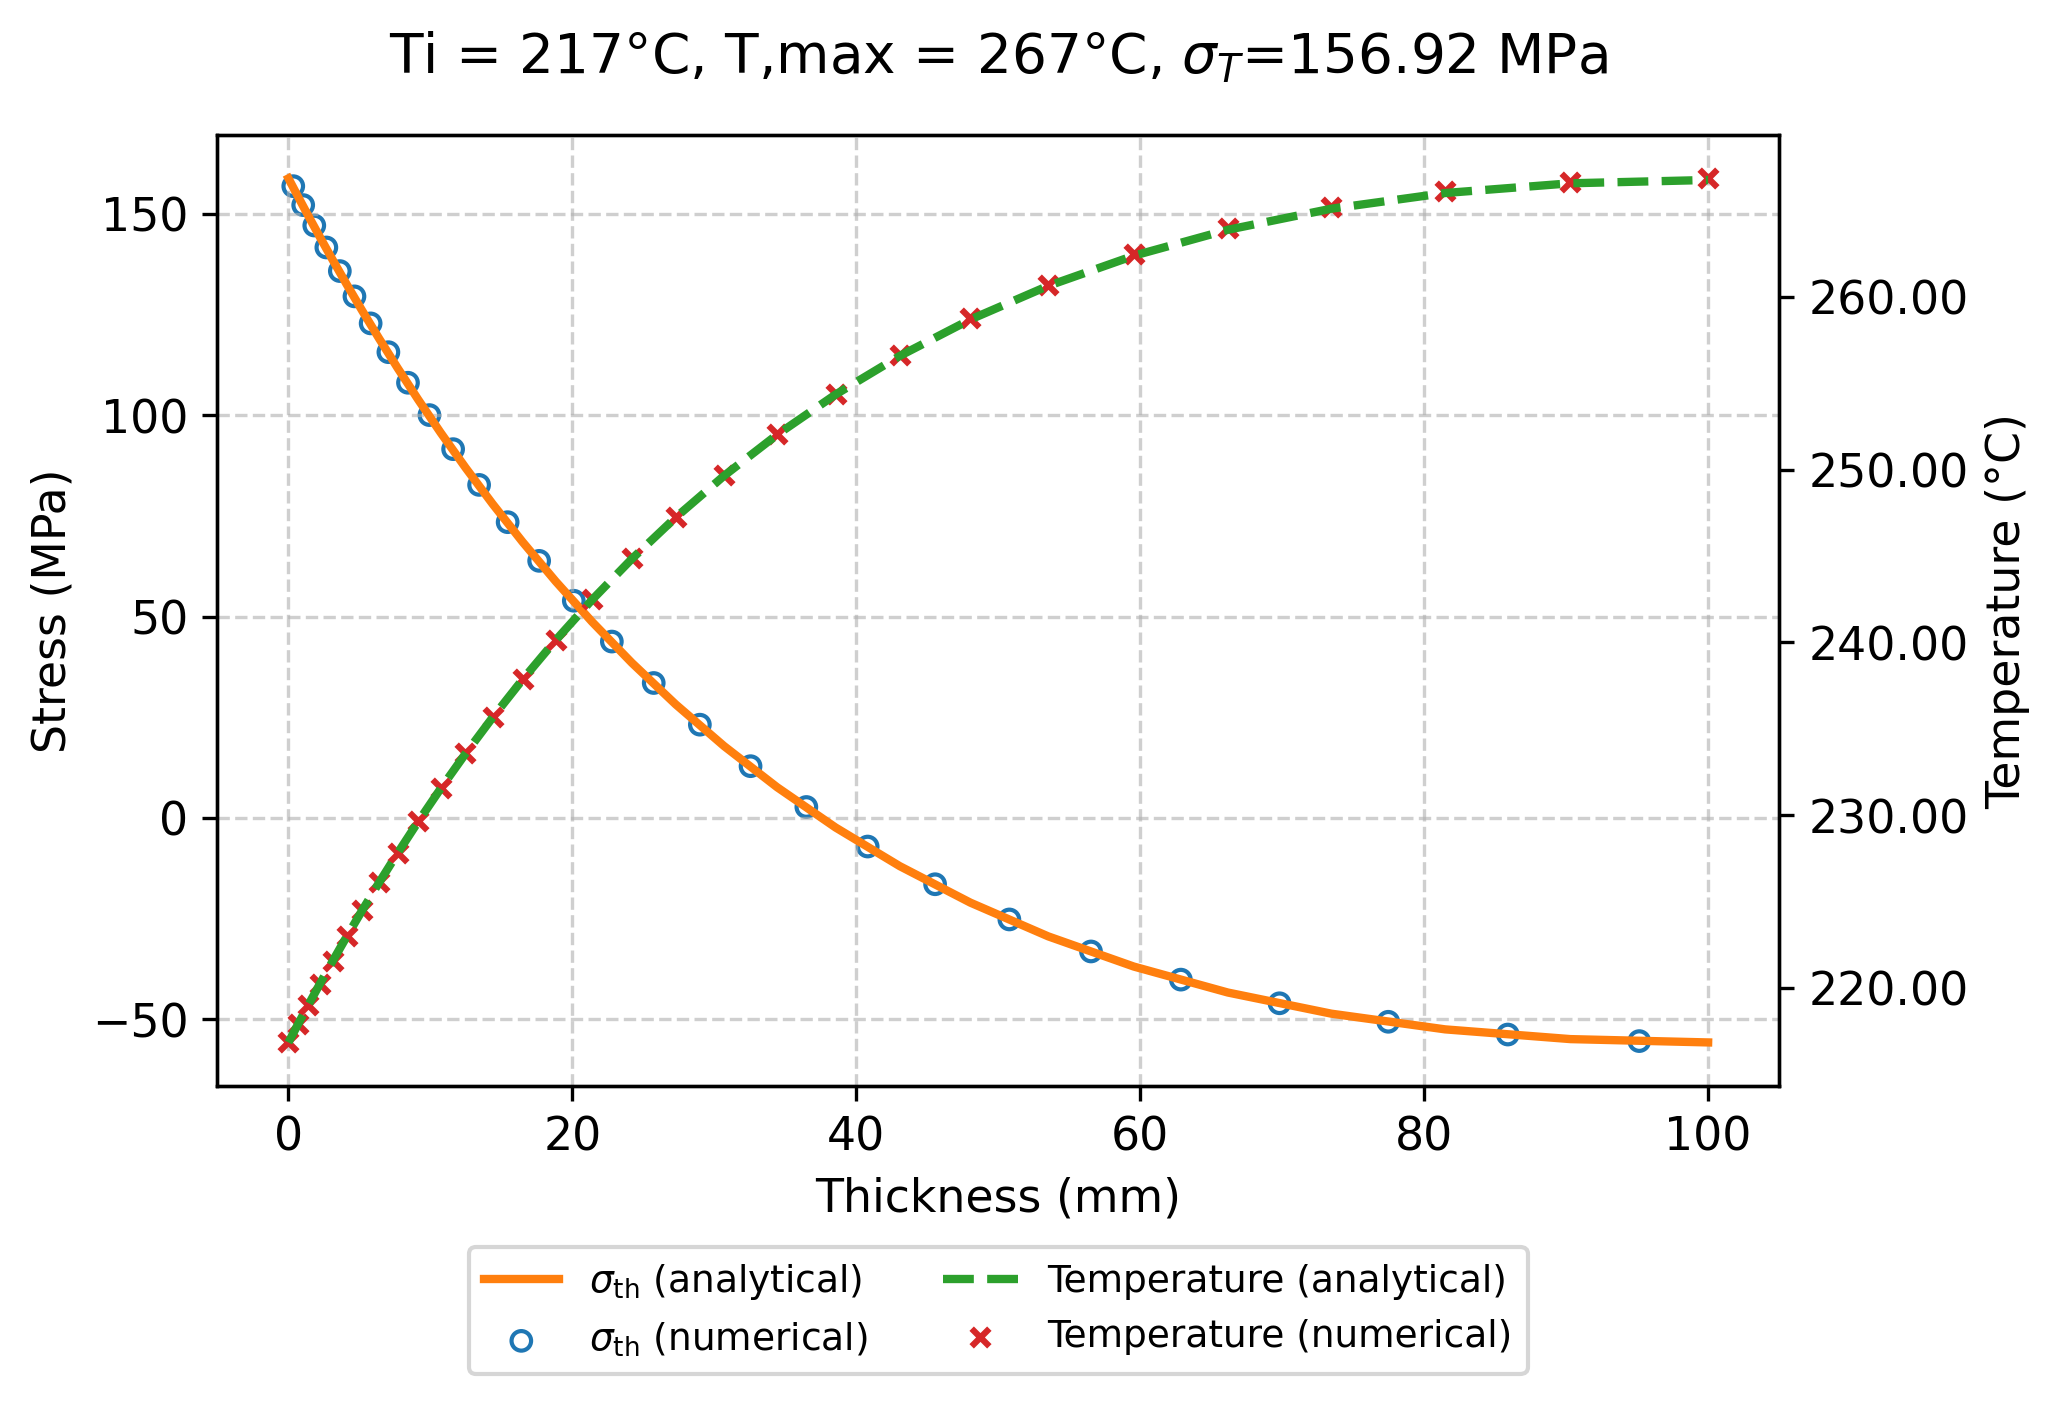
\includegraphics[height=0.74\textheight]{figures/thin_slab_stress_temperature.png}\\
  {\scriptsize thin slab: temperature and thermal stress, numerical vs analytical, across the thickness}
\end{frame}

\begin{frame}{Backup: automated creep-law discovery (EUCLID-style)}
  \scriptsize
  The differentiable machinery runs \alert{backwards} -- discover the constitutive
  law from noisy data, not just calibrate an assumed form.
  \begin{columns}[T]
    \begin{column}{0.45\textwidth}
      \textbf{Forward model -- implicit creep}
      \begin{itemize}
        \item Norton $\dot\varepsilon^{cr}_{eq} = A(T)\,\sigma_{eq}^{\,n}$,\;
              $A(T)=A_0\,e^{-Q/R_g T}$
        \item relaxation $\dot\sigma = -E\,\dot\varepsilon^{cr}_{eq}(\sigma)$,
              backward Euler
        \item each Newton step in \alert{forward-mode AD} $\Rightarrow$ exact
              $\partial\sigma_i/\partial\ln\beta_k$ through the implicit update
      \end{itemize}
      \textbf{Discovery}
      \begin{itemize}
        \item library $\dot\varepsilon^{cr}_{eq}=\sum_k \beta_k\,\phi_k(S)$,\;
              $\phi_k\!\in\!\{S, S^2, S^3, S^5, \sinh S\}$
        \item Gauss-Newton on $\ln\beta_k$, then \alert{backward elimination}
              (one-standard-error rule)
      \end{itemize}
    \end{column}
    \begin{column}{0.55\textwidth}
      \centering
      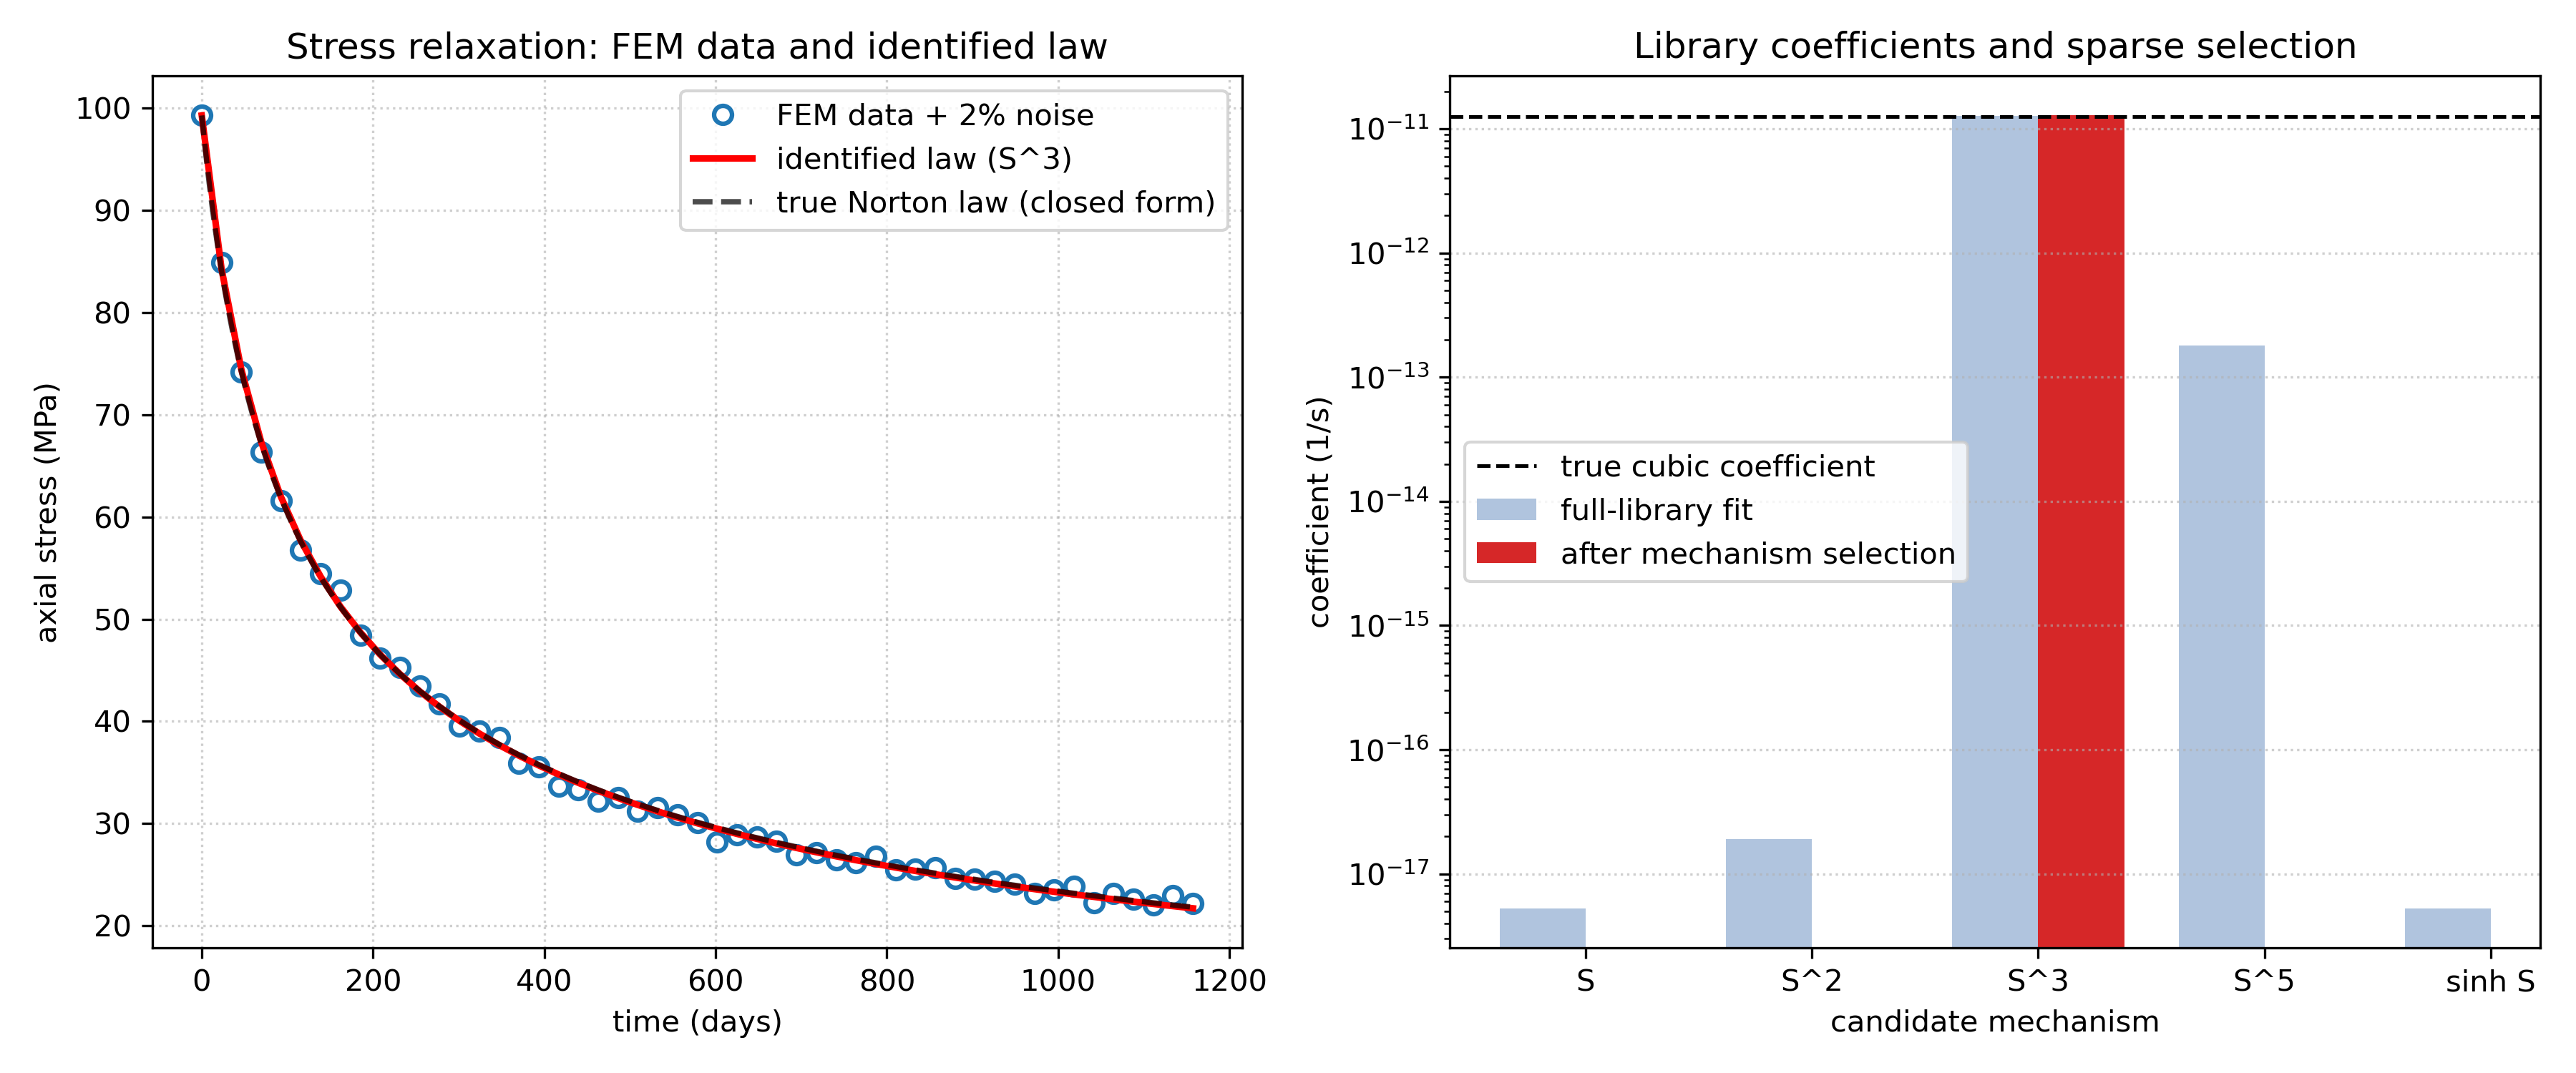
\includegraphics[width=\textwidth]{figures/creep_law_discovery.png}\\
      {\scriptsize left: noisy FEM data, identified $S^3$ law, closed-form Norton
      \;\textbar\; right: only the cubic mechanism survives selection (red)}
    \end{column}
  \end{columns}
  {\scriptsize From 2\% noisy data the \alert{cubic} Norton term is recovered alone
  -- 10/10 seeds, coefficient to \alert{1.7\%}; selection follows EUCLID (Flaschel et al.\ 2022).}
\end{frame}

\begin{frame}{Backup: penalty contact verified against analytical Lam\'e}
  \footnotesize
  \begin{columns}[T]
    \begin{column}{0.5\textwidth}
      \textbf{Contact across the closing gap}
      \begin{itemize}
        \item pellet heats, expands, \alert{closes the gap}, contacts the clad
        \item penalty $p = k_{pen}\langle -g\rangle_+$; traction $-p\,\mathbf{n}$ on both faces
        \item \alert{emergent} pressure; clad driven outward -- load transfer
        \item contact \alert{raises} gap conductance (Todreas Eq.~8.141) -- fuel cools
      \end{itemize}
      \vspace{0.2em}
      \centering
      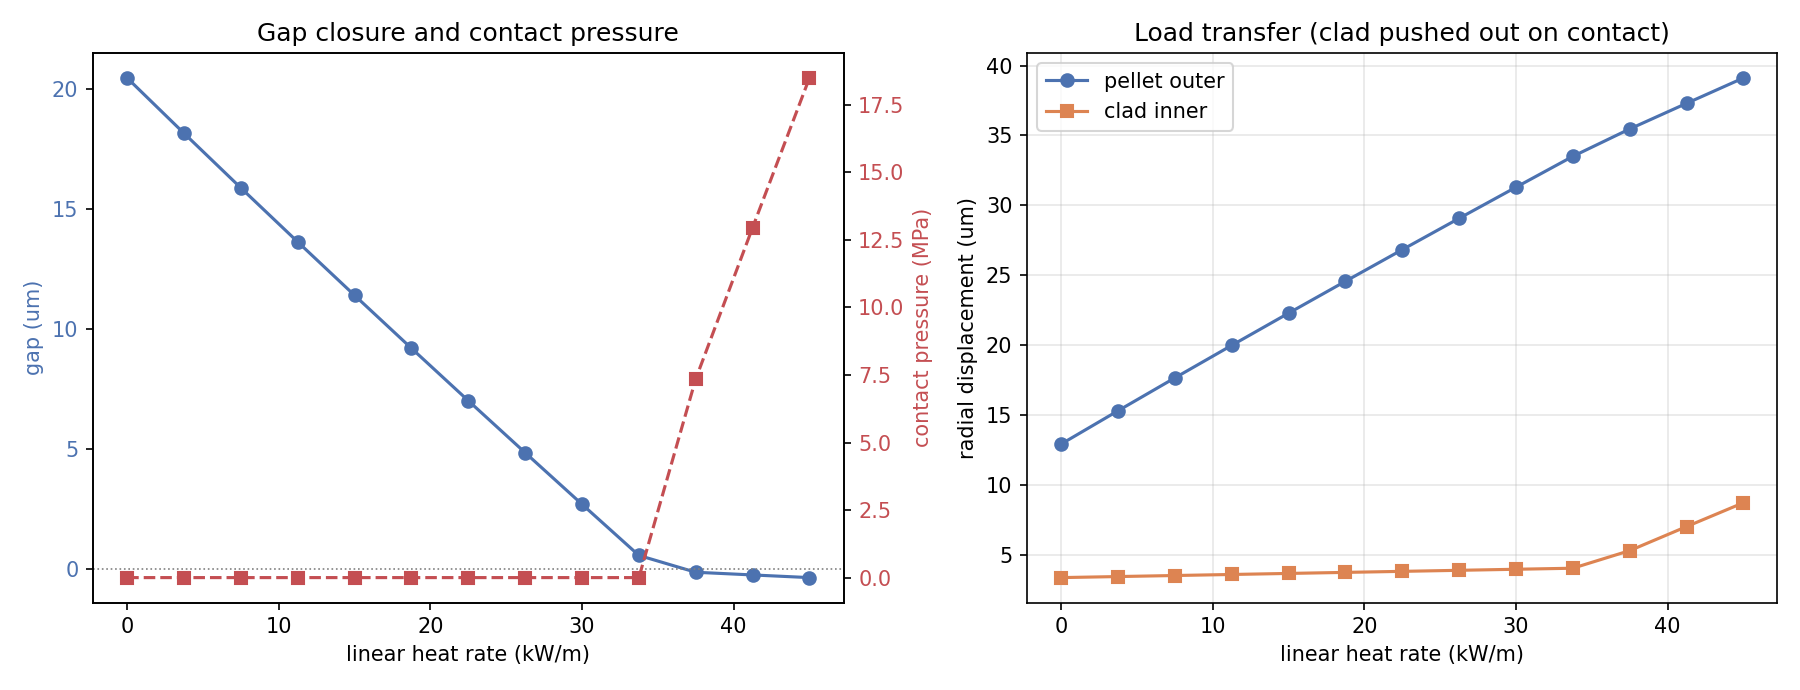
\includegraphics[height=3.1cm]{figures/pcmi_curves.png}
    \end{column}
    \begin{column}{0.5\textwidth}
      \textbf{Verified against analytical Lam\'e}
      \begin{itemize}
        \item uniform-$\Delta T$ interference fit: exact $\delta=\alpha_f(T-T_{ref})b - g_0$
        \item plane-stress regime \alert{confirmed} ($\sigma_{zz}\!\approx\!3\%$)
        \item penalty matches Lam\'e to \alert{3.5\%}
      \end{itemize}
      \vspace{0.2em}
      \centering
      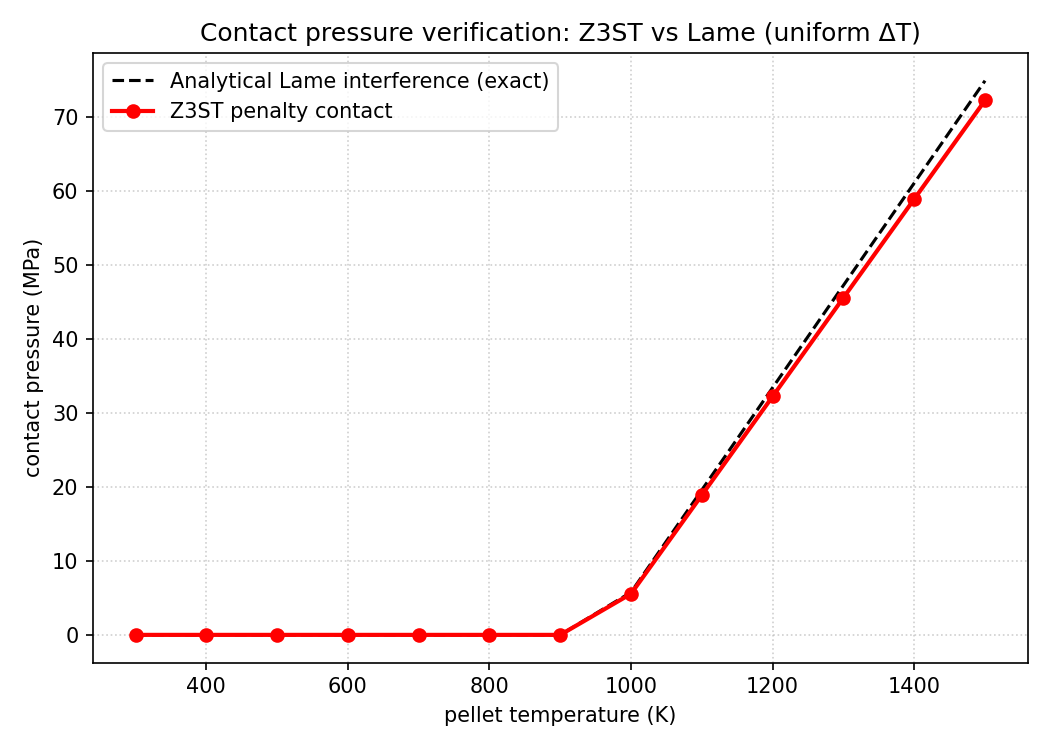
\includegraphics[height=3.1cm]{figures/pcmi_verification.png}
    \end{column}
  \end{columns}
  \vspace{0.2em}
  {\scriptsize Contact is an \alert{explicit} penalty for now -- the pressure is frozen
  from the previous iterate and the staggered loop drives it to a fixed point (no
  consistent contact tangent yet).}
\end{frame}

\begin{frame}{Backup: integral rod -- end-of-life stress state}
  \centering
  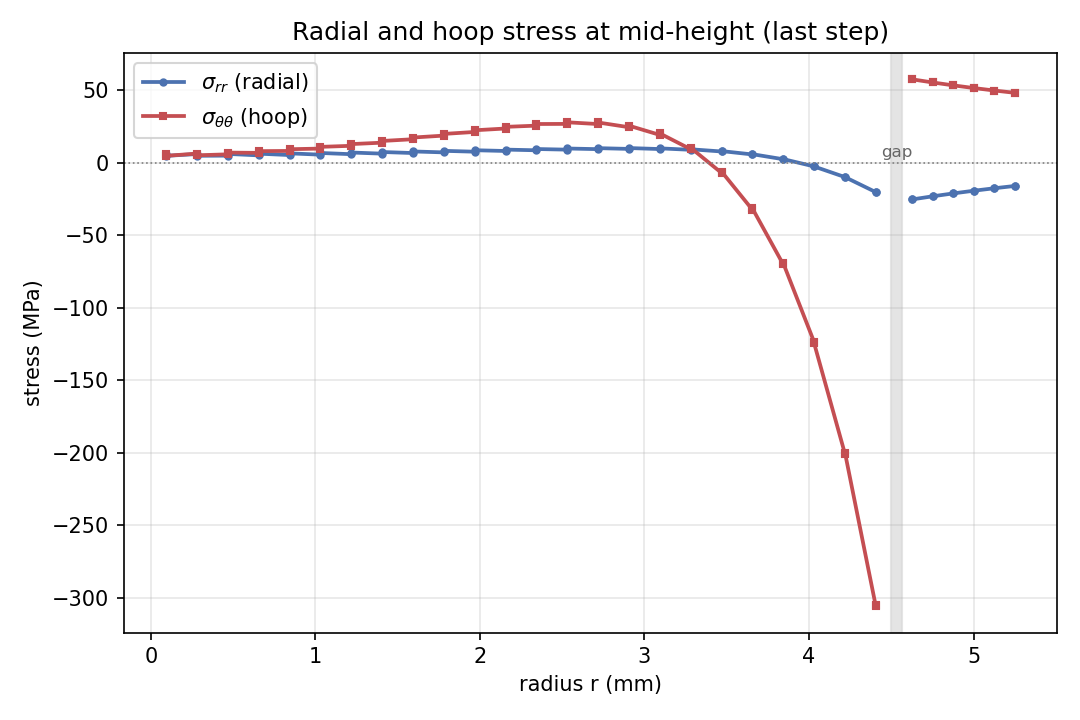
\includegraphics[height=0.66\textheight]{figures/pwr_rod_stress.png}\\[3pt]
  {\scriptsize Radial and hoop stress at mid-height at the end of the 1800-day
  history: the fuel surface carries a strong \alert{compressive hoop} stress
  ($\sim$-306\,MPa) and the cladding is left in mild tension -- the load-transfer
  state of an irradiated rod (shaded band = closed gap).}
\end{frame}

\begin{frame}{Backup: single-edge-notched shear -- a Miehe (2010) reproducer}
  \begin{columns}[T]
    \begin{column}{0.33\textwidth}\centering
      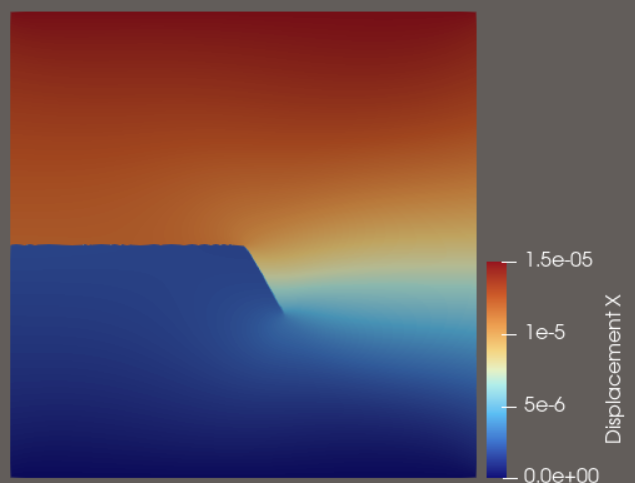
\includegraphics[width=\textwidth]{figures/sen_shear_ux.png}\\
      {\scriptsize imposed shear $u_x = 15\,\mu$m}
    \end{column}
    \begin{column}{0.33\textwidth}\centering
      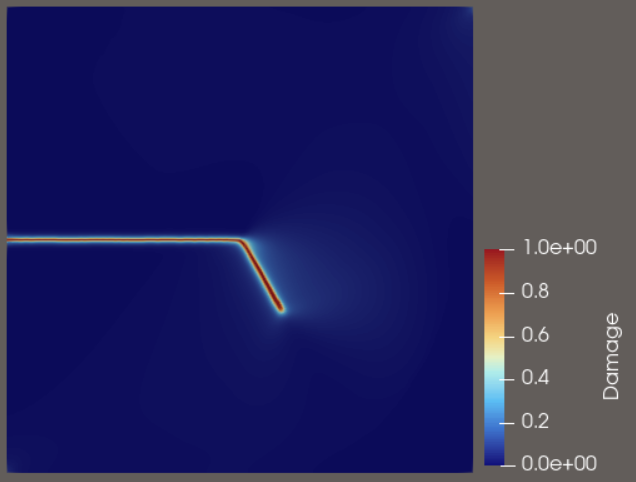
\includegraphics[width=\textwidth]{figures/sen_shear_damage.png}\\
      {\scriptsize phase-field damage: the curved crack path}
    \end{column}
    \begin{column}{0.33\textwidth}\centering
      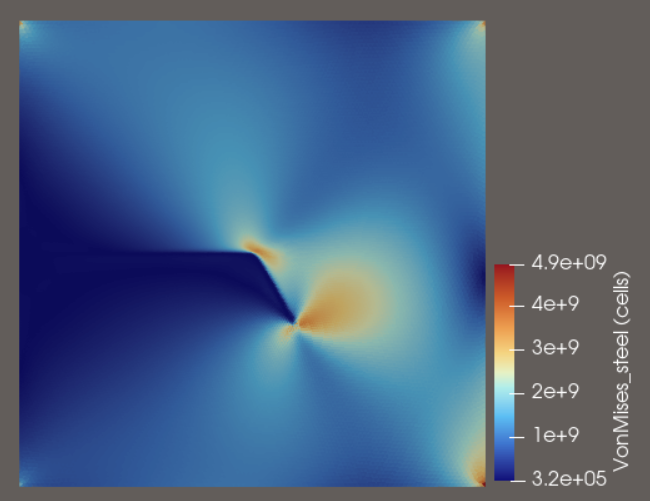
\includegraphics[width=\textwidth]{figures/sen_shear_vonmises.png}\\
      {\scriptsize von Mises stress at the crack tip}
    \end{column}
  \end{columns}
  \vspace{0.3em}
  \centering
  {\scriptsize mechanics $+$ phase-field damage; the curved crack reproduces
  Miehe et al., \textit{Comput. Methods Appl. Mech. Engrg.} 199 (2010) 2765--2778}
\end{frame}

\begin{frame}{Backup: hero case verified against McClenny (2022)}
  \centering
  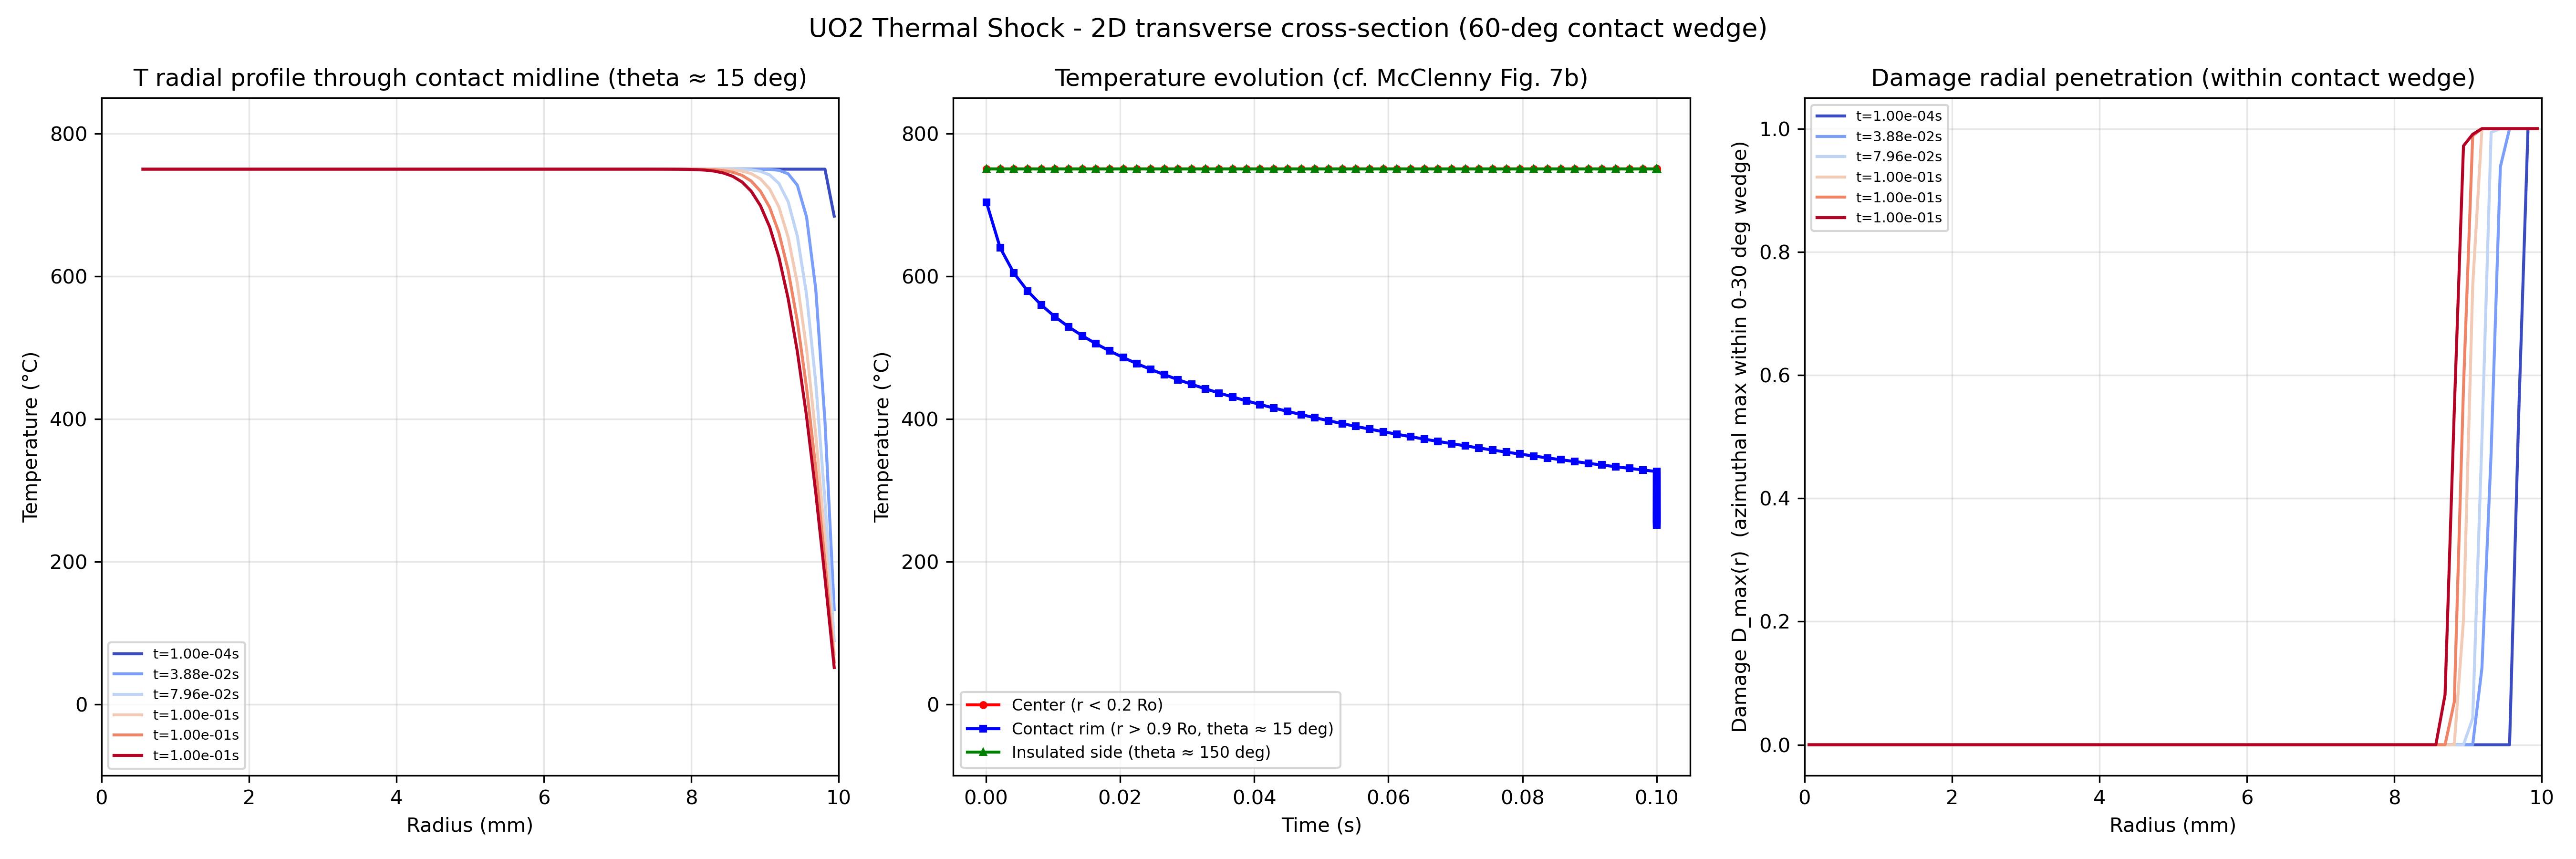
\includegraphics[width=0.70\textwidth]{figures/case14_results.png}\\[2pt]
  {\scriptsize radial $T$ profile, $T$ history, damage penetration -- cf.\ McClenny (2022), \textit{J.\ Nucl.\ Mater.} 565}\\[3pt]
  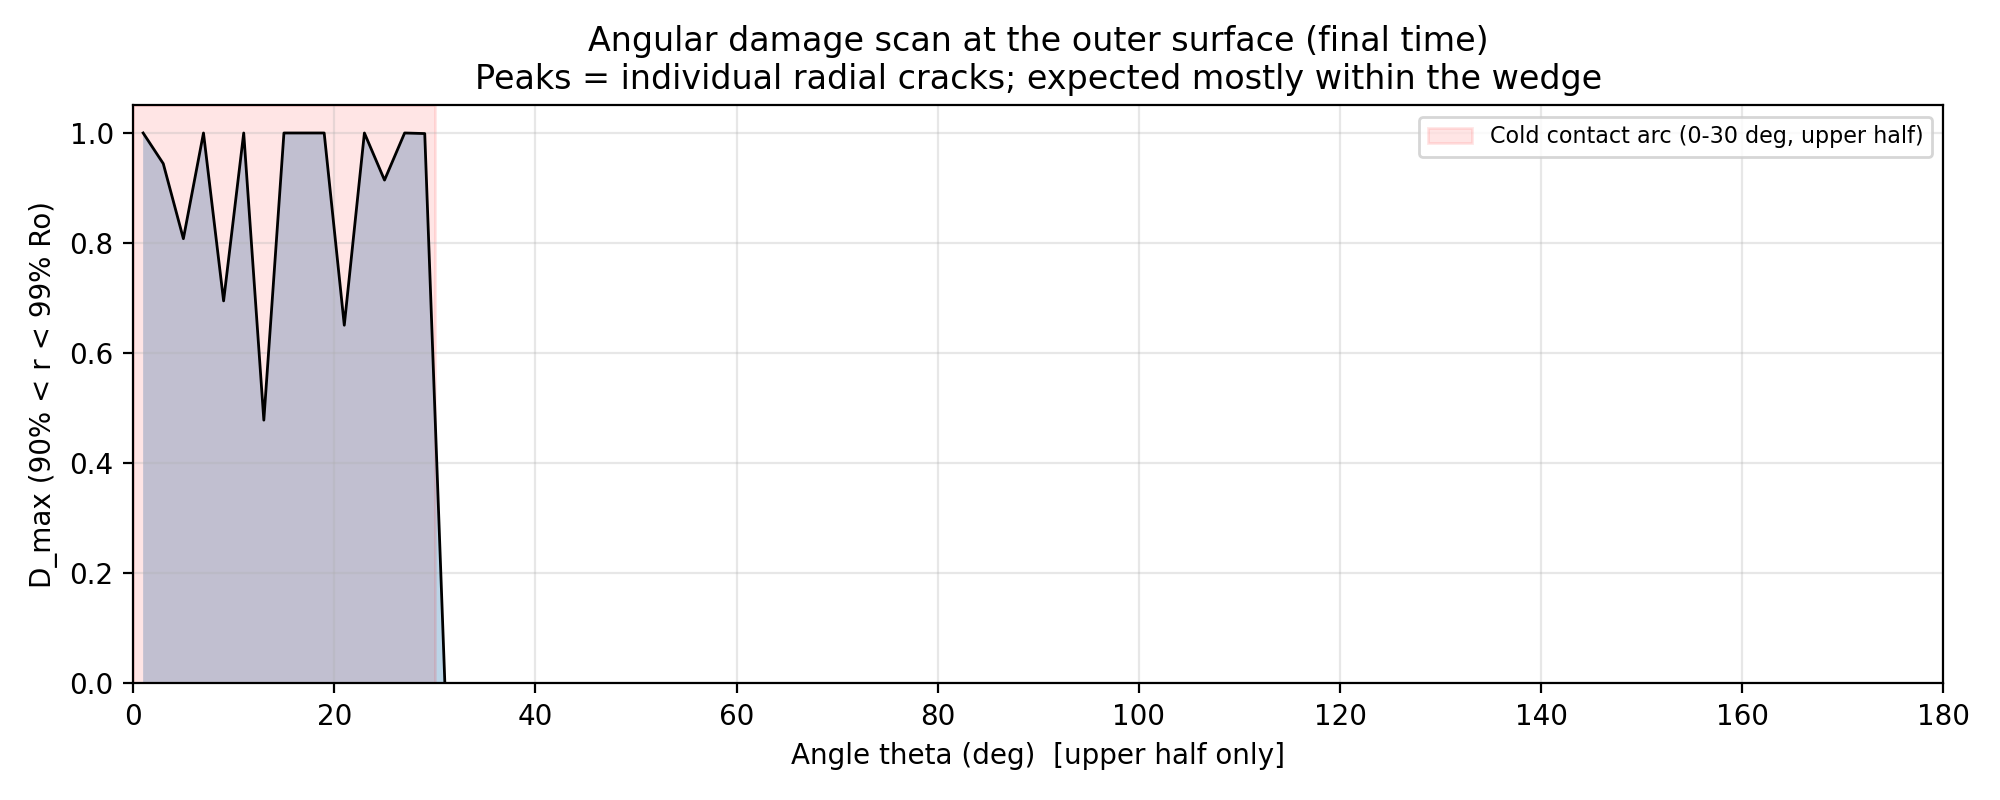
\includegraphics[width=0.40\textwidth]{figures/case14_damage_angular.png}\\[-1pt]
  {\scriptsize angular damage scan: \alert{discrete peaks = individual radial cracks}, confined to the cold-contact wedge}
\end{frame}

\end{document}
